\documentclass[1p]{elsarticle_modified}
%\bibliographystyle{elsarticle-num}

%\usepackage[colorlinks]{hyperref}
%\usepackage{abbrmath_seonhwa} %\Abb, \Ascr, \Acal ,\Abf, \Afrak
\usepackage{amsfonts}
\usepackage{amssymb}
\usepackage{amsmath}
\usepackage{amsthm}
\usepackage{scalefnt}
\usepackage{amsbsy}
\usepackage{kotex}
\usepackage{caption}
\usepackage{subfig}
\usepackage{color}
\usepackage{graphicx}
\usepackage{xcolor} %% white, black, red, green, blue, cyan, magenta, yellow
\usepackage{float}
\usepackage{setspace}
\usepackage{hyperref}

\usepackage{tikz}
\usetikzlibrary{arrows}

\usepackage{multirow}
\usepackage{array} % fixed length table
\usepackage{hhline}

%%%%%%%%%%%%%%%%%%%%%
\makeatletter
\renewcommand*\env@matrix[1][\arraystretch]{%
	\edef\arraystretch{#1}%
	\hskip -\arraycolsep
	\let\@ifnextchar\new@ifnextchar
	\array{*\c@MaxMatrixCols c}}
\makeatother %https://tex.stackexchange.com/questions/14071/how-can-i-increase-the-line-spacing-in-a-matrix
%%%%%%%%%%%%%%%

\usepackage[normalem]{ulem}

\newcommand{\msout}[1]{\ifmmode\text{\sout{\ensuremath{#1}}}\else\sout{#1}\fi}
%SOURCE: \msout is \stkout macro in https://tex.stackexchange.com/questions/20609/strikeout-in-math-mode

\newcommand{\cancel}[1]{
	\ifmmode
	{\color{red}\msout{#1}}
	\else
	{\color{red}\sout{#1}}
	\fi
}

\newcommand{\add}[1]{
	{\color{blue}\uwave{#1}}
}

\newcommand{\replace}[2]{
	\ifmmode
	{\color{red}\msout{#1}}{\color{blue}\uwave{#2}}
	\else
	{\color{red}\sout{#1}}{\color{blue}\uwave{#2}}
	\fi
}

\newcommand{\Sol}{\mathcal{S}} %segment
\newcommand{\D}{D} %diagram
\newcommand{\A}{\mathcal{A}} %arc


%%%%%%%%%%%%%%%%%%%%%%%%%%%%%5 test

\def\sl{\operatorname{\textup{SL}}(2,\Cbb)}
\def\psl{\operatorname{\textup{PSL}}(2,\Cbb)}
\def\quan{\mkern 1mu \triangleright \mkern 1mu}

\theoremstyle{definition}
\newtheorem{thm}{Theorem}[section]
\newtheorem{prop}[thm]{Proposition}
\newtheorem{lem}[thm]{Lemma}
\newtheorem{ques}[thm]{Question}
\newtheorem{cor}[thm]{Corollary}
\newtheorem{defn}[thm]{Definition}
\newtheorem{exam}[thm]{Example}
\newtheorem{rmk}[thm]{Remark}
\newtheorem{alg}[thm]{Algorithm}

\newcommand{\I}{\sqrt{-1}}
\begin{document}

%\begin{frontmatter}
%
%\title{Boundary parabolic representations of knots up to 8 crossings}
%
%%% Group authors per affiliation:
%\author{Yunhi Cho} 
%\address{Department of Mathematics, University of Seoul, Seoul, Korea}
%\ead{yhcho@uos.ac.kr}
%
%
%\author{Seonhwa Kim} %\fnref{s_kim}}
%\address{Center for Geometry and Physics, Institute for Basic Science, Pohang, 37673, Korea}
%\ead{ryeona17@ibs.re.kr}
%
%\author{Hyuk Kim}
%\address{Department of Mathematical Sciences, Seoul National University, Seoul 08826, Korea}
%\ead{hyukkim@snu.ac.kr}
%
%\author{Seokbeom Yoon}
%\address{Department of Mathematical Sciences, Seoul National University, Seoul, 08826,  Korea}
%\ead{sbyoon15@snu.ac.kr}
%
%\begin{abstract}
%We find all boundary parabolic representation of knots up to 8 crossings.
%
%\end{abstract}
%\begin{keyword}
%    \MSC[2010] 57M25 
%\end{keyword}
%
%\end{frontmatter}

%\linenumbers
%\tableofcontents
%
\newcommand\colored[1]{\textcolor{white}{\rule[-0.35ex]{0.8em}{1.4ex}}\kern-0.8em\color{red} #1}%
%\newcommand\colored[1]{\textcolor{white}{ #1}\kern-2.17ex	\textcolor{white}{ #1}\kern-1.81ex	\textcolor{white}{ #1}\kern-2.15ex\color{red}#1	}

{\Large $\underline{12a_{0692}~(K12a_{0692})}$}

\setlength{\tabcolsep}{10pt}
\renewcommand{\arraystretch}{1.6}
\vspace{1cm}\begin{tabular}{m{100pt}>{\centering\arraybackslash}m{274pt}}
\multirow{5}{120pt}{
	\centering
	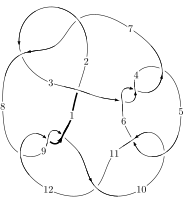
\includegraphics[width=112pt]{../../../GIT/diagram.site/Diagrams/png/1493_12a_0692.png}\\
\ \ \ A knot diagram\footnotemark}&
\allowdisplaybreaks
\textbf{Linearized knot diagam} \\
\cline{2-2}
 &
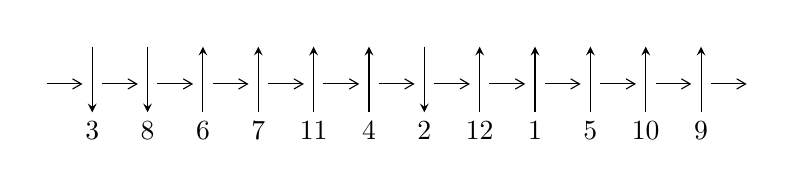
\begin{tikzpicture}[x=20pt, y=17pt]
	% nodes
	\node (C0) at (0, 0) {};
	\node (C1) at (1, 0) {};
	\node (C1U) at (1, +1) {};
	\node (C1D) at (1, -1) {3};

	\node (C2) at (2, 0) {};
	\node (C2U) at (2, +1) {};
	\node (C2D) at (2, -1) {8};

	\node (C3) at (3, 0) {};
	\node (C3U) at (3, +1) {};
	\node (C3D) at (3, -1) {6};

	\node (C4) at (4, 0) {};
	\node (C4U) at (4, +1) {};
	\node (C4D) at (4, -1) {7};

	\node (C5) at (5, 0) {};
	\node (C5U) at (5, +1) {};
	\node (C5D) at (5, -1) {11};

	\node (C6) at (6, 0) {};
	\node (C6U) at (6, +1) {};
	\node (C6D) at (6, -1) {4};

	\node (C7) at (7, 0) {};
	\node (C7U) at (7, +1) {};
	\node (C7D) at (7, -1) {2};

	\node (C8) at (8, 0) {};
	\node (C8U) at (8, +1) {};
	\node (C8D) at (8, -1) {12};

	\node (C9) at (9, 0) {};
	\node (C9U) at (9, +1) {};
	\node (C9D) at (9, -1) {1};

	\node (C10) at (10, 0) {};
	\node (C10U) at (10, +1) {};
	\node (C10D) at (10, -1) {5};

	\node (C11) at (11, 0) {};
	\node (C11U) at (11, +1) {};
	\node (C11D) at (11, -1) {10};

	\node (C12) at (12, 0) {};
	\node (C12U) at (12, +1) {};
	\node (C12D) at (12, -1) {9};
	\node (C13) at (13, 0) {};

	% arrows
	\draw[->,>={angle 60}]
	(C0) edge (C1) (C1) edge (C2) (C2) edge (C3) (C3) edge (C4) (C4) edge (C5) (C5) edge (C6) (C6) edge (C7) (C7) edge (C8) (C8) edge (C9) (C9) edge (C10) (C10) edge (C11) (C11) edge (C12) (C12) edge (C13) ;	\draw[->,>=stealth]
	(C1U) edge (C1D) (C2U) edge (C2D) (C3D) edge (C3U) (C4D) edge (C4U) (C5D) edge (C5U) (C6D) edge (C6U) (C7U) edge (C7D) (C8D) edge (C8U) (C9D) edge (C9U) (C10D) edge (C10U) (C11D) edge (C11U) (C12D) edge (C12U) ;
	\end{tikzpicture} \\
\hhline{~~} \\& 
\textbf{Solving Sequence} \\ \cline{2-2} 
 &
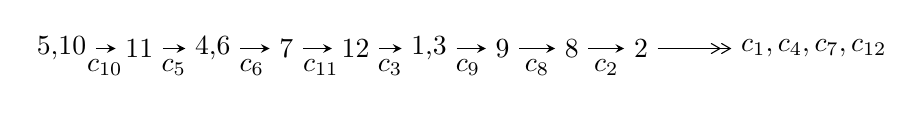
\begin{tikzpicture}[x=25pt, y=7pt]
	% node
	\node (A0) at (-1/8, 0) {5,10};
	\node (A1) at (1, 0) {11};
	\node (A2) at (33/16, 0) {4,6};
	\node (A3) at (25/8, 0) {7};
	\node (A4) at (33/8, 0) {12};
	\node (A5) at (83/16, 0) {1,3};
	\node (A6) at (25/4, 0) {9};
	\node (A7) at (29/4, 0) {8};
	\node (A8) at (33/4, 0) {2};
	\node (C1) at (1/2, -1) {$c_{10}$};
	\node (C2) at (3/2, -1) {$c_{5}$};
	\node (C3) at (21/8, -1) {$c_{6}$};
	\node (C4) at (29/8, -1) {$c_{11}$};
	\node (C5) at (37/8, -1) {$c_{3}$};
	\node (C6) at (23/4, -1) {$c_{9}$};
	\node (C7) at (27/4, -1) {$c_{8}$};
	\node (C8) at (31/4, -1) {$c_{2}$};
	\node (A9) at (43/4, 0) {$c_{1},c_{4},c_{7},c_{12}$};

	% edge
	\draw[->,>=stealth]	
	(A0) edge (A1) (A1) edge (A2) (A2) edge (A3) (A3) edge (A4) (A4) edge (A5) (A5) edge (A6) (A6) edge (A7) (A7) edge (A8) ;
	\draw[->>,>={angle 60}]	
	(A8) edge (A9);
\end{tikzpicture} \\ 

\end{tabular} \\

\footnotetext{
The image of knot diagram is generated by the software ``\textbf{Draw programme}" developed by Andrew Bartholomew(\url{http://www.layer8.co.uk/maths/draw/index.htm\#Running-draw}), where we modified some parts for our purpose(\url{https://github.com/CATsTAILs/LinksPainter}).
}\phantom \\ \newline 
\centering \textbf{Ideals for irreducible components\footnotemark of $X_{\text{par}}$} 
 
\begin{align*}
I^u_{1}&=\langle 
1645225595 u^{22}+1403326418 u^{21}+\cdots+92459847924 d+6684425356,\\
\phantom{I^u_{1}}&\phantom{= \langle  }-57765211 u^{22}+603981722 u^{21}+\cdots+61639898616 c-10033883264,\\
\phantom{I^u_{1}}&\phantom{= \langle  }764605576 u^{22}+1158469312 u^{21}+\cdots+46229923962 b+3650149526,\\
\phantom{I^u_{1}}&\phantom{= \langle  }1181950799 u^{22}+2420172188 u^{21}+\cdots+61639898616 a-56011531544,\\
\phantom{I^u_{1}}&\phantom{= \langle  }u^{23}+2 u^{22}+\cdots-4 u^2+8\rangle \\
I^u_{2}&=\langle 
-4 u^3 a+7 u^2 a-6 u^3- a u+7 u^2+7 d+2 a-12 u+10,\\
\phantom{I^u_{2}}&\phantom{= \langle  }-2 u^3 a+7 u^2 a-3 u^3-4 a u+7 u^2+7 c+a-6 u+5,\;u^3 a+5 u^3+2 a u-7 u^2+7 b-4 a+3 u+1,\\
\phantom{I^u_{2}}&\phantom{= \langle  }- u^3 a+2 u^2 a-2 u^3+a^2-2 a u+4 u^2-2 u+1,\;u^4-2 u^3+2 u^2- u+1\rangle \\
I^u_{3}&=\langle 
u^7+u^6-2 u^5- u^4+2 u^3+2 u^2+d-2 u-1,\;u^6- u^4+2 u^2+c-1,\\
\phantom{I^u_{3}}&\phantom{= \langle  }-22 u^7 a-11 u^6 a-20 u^7+9 u^5 a-10 u^6+21 u^4 a+25 u^5-14 u^3 a+9 u^4-43 u^3+37 b+7 a+37 u+40,\\
\phantom{I^u_{3}}&\phantom{= \langle  }-4 u^7 a+2 u^7+\cdots+8 a-2,\;u^8+u^7- u^6-2 u^5+u^4+2 u^3-2 u-1\rangle \\
I^u_{4}&=\langle 
u^7 c-2 u^7- u^5 c- u^6- u^4 c+2 u^5+2 u^3 c+2 u^4+2 u^2 c-3 u^3- u^2+d-3 c+u+3,\\
\phantom{I^u_{4}}&\phantom{= \langle  }2 u^7 c+u^6 c- u^7-2 u^5 c-3 u^4 c+2 u^5+2 u^3 c+u^4+2 u^2 c-3 u^3+c^2- u^2-3 c+u+2,\;- u^5+u^3+b- u,\\
\phantom{I^u_{4}}&\phantom{= \langle  }u^3+a,\;u^8+u^7- u^6-2 u^5+u^4+2 u^3-2 u-1\rangle \\
I^u_{5}&=\langle 
u^7+u^6-2 u^5- u^4+2 u^3+2 u^2+d-2 u-1,\;u^6- u^4+2 u^2+c-1,\;- u^5+u^3+b- u,\;u^3+a,\\
\phantom{I^u_{5}}&\phantom{= \langle  }u^8+u^7- u^6-2 u^5+u^4+2 u^3-2 u-1\rangle \\
I^u_{6}&=\langle 
u^4 a-3 u^5+u^3 a+u^4- u^2 a+4 u^3+a u-5 u^2+d+2 a- u+5,\\
\phantom{I^u_{6}}&\phantom{= \langle  }2 u^5 a- u^5-2 u^3 a+u^4+2 u^2 a+3 u^3+2 a u-3 u^2+2 c-2 a+u+4,\\
\phantom{I^u_{6}}&\phantom{= \langle  }u^4 a- u^5+u^4+u^3+a u-2 u^2+b+u+2,\\
\phantom{I^u_{6}}&\phantom{= \langle  }-3 u^5 a- u^4 a- u^5+3 u^3 a- u^4-3 u^2 a- u^3+2 a^2-3 a u+u^2+4 a- u-2,\\
\phantom{I^u_{6}}&\phantom{= \langle  }u^6- u^5- u^4+3 u^3- u^2-2 u+2\rangle \\
\\
I^v_{1}&=\langle 
a,\;d+1,\;c- a+1,\;b+1,\;v+1\rangle \\
I^v_{2}&=\langle 
a,\;d,\;c-1,\;b+1,\;v-1\rangle \\
I^v_{3}&=\langle 
c,\;d-1,\;b,\;a-1,\;v-1\rangle \\
I^v_{4}&=\langle 
a,\;d a+c- v-1,\;d v-1,\;c v- v^2+a- v,\;b+1\rangle \\
\end{align*}
\raggedright * 9 irreducible components of $\dim_{\mathbb{C}}=0$, with total 86 representations.\\
\raggedright * 1 irreducible components of $\dim_{\mathbb{C}}=1$ \\
\footnotetext{All coefficients of polynomials are rational numbers. But the coefficients are sometimes approximated in decimal forms when there is not enough margin.}
\newpage
\renewcommand{\arraystretch}{1}
\centering \section*{I. $I^u_{1}= \langle 1.65\times10^{9} u^{22}+1.40\times10^{9} u^{21}+\cdots+9.25\times10^{10} d+6.68\times10^{9},\;-5.78\times10^{7} u^{22}+6.04\times10^{8} u^{21}+\cdots+6.16\times10^{10} c-1.00\times10^{10},\;7.65\times10^{8} u^{22}+1.16\times10^{9} u^{21}+\cdots+4.62\times10^{10} b+3.65\times10^{9},\;1.18\times10^{9} u^{22}+2.42\times10^{9} u^{21}+\cdots+6.16\times10^{10} a-5.60\times10^{10},\;u^{23}+2 u^{22}+\cdots-4 u^2+8 \rangle$}
\flushleft \textbf{(i) Arc colorings}\\
\begin{tabular}{m{7pt} m{180pt} m{7pt} m{180pt} }
\flushright $a_{5}=$&$\begin{pmatrix}0\\u\end{pmatrix}$ \\
\flushright $a_{10}=$&$\begin{pmatrix}1\\0\end{pmatrix}$ \\
\flushright $a_{11}=$&$\begin{pmatrix}1\\- u^2\end{pmatrix}$ \\
\flushright $a_{4}=$&$\begin{pmatrix}0.000937140 u^{22}-0.00979855 u^{21}+\cdots-0.137025 u+0.162782\\-0.0177939 u^{22}-0.0151777 u^{21}+\cdots+0.995143 u-0.0722954\end{pmatrix}$ \\
\flushright $a_{6}=$&$\begin{pmatrix}u\\- u^3+u\end{pmatrix}$ \\
\flushright $a_{7}=$&$\begin{pmatrix}-0.00986955 u^{22}-0.00319991 u^{21}+\cdots+1.12467 u-0.141695\\-0.000912892 u^{22}-0.00272992 u^{21}+\cdots+0.908690 u+0.153401\end{pmatrix}$ \\
\flushright $a_{12}=$&$\begin{pmatrix}- u^2+1\\- u^2\end{pmatrix}$ \\
\flushright $a_{1}=$&$\begin{pmatrix}-0.0191751 u^{22}-0.0392631 u^{21}+\cdots+0.119456 u+0.908690\\-0.0165392 u^{22}-0.0250589 u^{21}+\cdots+0.141695 u-0.0789564\end{pmatrix}$ \\
\flushright $a_{3}=$&$\begin{pmatrix}0.00895666 u^{22}+0.000469997 u^{21}+\cdots-0.215981 u+0.295096\\-0.0120388 u^{22}-0.00566656 u^{21}+\cdots+0.980343 u+0.0138542\end{pmatrix}$ \\
\flushright $a_{9}=$&$\begin{pmatrix}0.00903693 u^{22}+0.000279913 u^{21}+\cdots-0.185021 u+0.995143\\0.0116728 u^{22}+0.0144841 u^{21}+\cdots-0.162782 u+0.00749712\end{pmatrix}$ \\
\flushright $a_{8}=$&$\begin{pmatrix}-0.00173177 u^{22}-0.0155024 u^{21}+\cdots-0.175640 u+0.980343\\0.0174433 u^{22}+0.0237607 u^{21}+\cdots-0.295096 u+0.0716533\end{pmatrix}$ \\
\flushright $a_{2}=$&$\begin{pmatrix}0.0171752 u^{22}+0.0429380 u^{21}+\cdots-0.0481132 u+1.21453\\0.0545823 u^{22}+0.0631700 u^{21}+\cdots+0.915273 u+0.299257\end{pmatrix}$\\&\end{tabular}
\flushleft \textbf{(ii) Obstruction class $= -1$}\\~\\
\flushleft \textbf{(iii) Cusp Shapes $= \frac{15567855023}{46229923962} u^{22}+\frac{8703838979}{46229923962} u^{21}+\cdots-\frac{168604101146}{23114961981} u+\frac{87470148380}{23114961981}$}\\~\\
\newpage\renewcommand{\arraystretch}{1}
\flushleft \textbf{(iv) u-Polynomials at the component}\newline \\
\begin{tabular}{m{50pt}|m{274pt}}
Crossings & \hspace{64pt}u-Polynomials at each crossing \\
\hline $$\begin{aligned}c_{1}\end{aligned}$$&$\begin{aligned}
&u^{23}+10 u^{22}+\cdots+88 u+16
\end{aligned}$\\
\hline $$\begin{aligned}c_{2},c_{7}\end{aligned}$$&$\begin{aligned}
&u^{23}-2 u^{22}+\cdots+8 u-4
\end{aligned}$\\
\hline $$\begin{aligned}c_{3},c_{4},c_{6}\\c_{8},c_{9},c_{12}\end{aligned}$$&$\begin{aligned}
&u^{23}+2 u^{22}+\cdots- u-1
\end{aligned}$\\
\hline $$\begin{aligned}c_{5},c_{10}\end{aligned}$$&$\begin{aligned}
&u^{23}-2 u^{22}+\cdots+4 u^2-8
\end{aligned}$\\
\hline $$\begin{aligned}c_{11}\end{aligned}$$&$\begin{aligned}
&u^{23}-6 u^{22}+\cdots+64 u-64
\end{aligned}$\\
\hline
\end{tabular}\\~\\
\newpage\renewcommand{\arraystretch}{1}
\flushleft \textbf{(v) Riley Polynomials at the component}\newline \\
\begin{tabular}{m{50pt}|m{274pt}}
Crossings & \hspace{64pt}Riley Polynomials at each crossing \\
\hline $$\begin{aligned}c_{1}\end{aligned}$$&$\begin{aligned}
&y^{23}+6 y^{22}+\cdots+1824 y-256
\end{aligned}$\\
\hline $$\begin{aligned}c_{2},c_{7}\end{aligned}$$&$\begin{aligned}
&y^{23}-10 y^{22}+\cdots+88 y-16
\end{aligned}$\\
\hline $$\begin{aligned}c_{3},c_{4},c_{6}\\c_{8},c_{9},c_{12}\end{aligned}$$&$\begin{aligned}
&y^{23}-24 y^{22}+\cdots-9 y-1
\end{aligned}$\\
\hline $$\begin{aligned}c_{5},c_{10}\end{aligned}$$&$\begin{aligned}
&y^{23}-6 y^{22}+\cdots+64 y-64
\end{aligned}$\\
\hline $$\begin{aligned}c_{11}\end{aligned}$$&$\begin{aligned}
&y^{23}+10 y^{22}+\cdots-6144 y-4096
\end{aligned}$\\
\hline
\end{tabular}\\~\\
\newpage\flushleft \textbf{(vi) Complex Volumes and Cusp Shapes}
$$\begin{array}{c|c|c}  
\text{Solutions to }I^u_{1}& \I (\text{vol} + \sqrt{-1}CS) & \text{Cusp shape}\\
 \hline 
\begin{aligned}
u &= -0.758227 + 0.807207 I \\
a &= \phantom{-}0.65983 + 1.27023 I \\
b &= \phantom{-}0.027613 + 0.769755 I \\
c &= -0.393809 - 0.363183 I \\
d &= -0.468974 - 0.379047 I\end{aligned}
 & -5.90461 + 1.36538 I & -0.279938 - 0.826772 I \\ \hline\begin{aligned}
u &= -0.758227 - 0.807207 I \\
a &= \phantom{-}0.65983 - 1.27023 I \\
b &= \phantom{-}0.027613 - 0.769755 I \\
c &= -0.393809 + 0.363183 I \\
d &= -0.468974 + 0.379047 I\end{aligned}
 & -5.90461 - 1.36538 I & -0.279938 + 0.826772 I \\ \hline\begin{aligned}
u &= \phantom{-}0.830705 + 0.204801 I \\
a &= \phantom{-}0.205779 - 0.701670 I \\
b &= -0.423290 - 0.486601 I \\
c &= -0.049881 - 0.483602 I \\
d &= \phantom{-}0.434396 + 0.280584 I\end{aligned}
 & \phantom{-}0.25505 + 3.01929 I & \phantom{-}7.24264 - 9.08374 I \\ \hline\begin{aligned}
u &= \phantom{-}0.830705 - 0.204801 I \\
a &= \phantom{-}0.205779 + 0.701670 I \\
b &= -0.423290 + 0.486601 I \\
c &= -0.049881 + 0.483602 I \\
d &= \phantom{-}0.434396 - 0.280584 I\end{aligned}
 & \phantom{-}0.25505 - 3.01929 I & \phantom{-}7.24264 + 9.08374 I \\ \hline\begin{aligned}
u &= \phantom{-}0.112218 + 1.144740 I \\
a &= -0.975240 + 0.062634 I \\
b &= -1.392930 + 0.053326 I \\
c &= -0.03579 + 1.68894 I \\
d &= \phantom{-}0.42369 + 2.68034 I\end{aligned}
 & \phantom{-}8.23677 - 2.50119 I & \phantom{-}13.28602 + 3.12140 I \\ \hline\begin{aligned}
u &= \phantom{-}0.112218 - 1.144740 I \\
a &= -0.975240 - 0.062634 I \\
b &= -1.392930 - 0.053326 I \\
c &= -0.03579 - 1.68894 I \\
d &= \phantom{-}0.42369 - 2.68034 I\end{aligned}
 & \phantom{-}8.23677 + 2.50119 I & \phantom{-}13.28602 - 3.12140 I\\
 \hline 
 \end{array}$$\newpage$$\begin{array}{c|c|c}  
\text{Solutions to }I^u_{1}& \I (\text{vol} + \sqrt{-1}CS) & \text{Cusp shape}\\
 \hline 
\begin{aligned}
u &= \phantom{-}0.561270 + 1.026650 I \\
a &= -0.909276 + 0.320219 I \\
b &= -1.332320 + 0.271054 I \\
c &= -0.15598 + 1.57216 I \\
d &= \phantom{-}1.88354 + 1.80349 I\end{aligned}
 & \phantom{-}5.56899 - 4.43236 I & \phantom{-}12.33564 + 2.61344 I \\ \hline\begin{aligned}
u &= \phantom{-}0.561270 - 1.026650 I \\
a &= -0.909276 - 0.320219 I \\
b &= -1.332320 - 0.271054 I \\
c &= -0.15598 - 1.57216 I \\
d &= \phantom{-}1.88354 - 1.80349 I\end{aligned}
 & \phantom{-}5.56899 + 4.43236 I & \phantom{-}12.33564 - 2.61344 I \\ \hline\begin{aligned}
u &= -0.972761 + 0.735330 I \\
a &= \phantom{-}0.435991 + 1.279060 I \\
b &= -0.128148 + 0.852673 I \\
c &= -0.356815 - 0.494380 I \\
d &= -0.010338 - 0.309906 I\end{aligned}
 & -5.23569 - 7.16228 I & \phantom{-}1.72036 + 6.58026 I \\ \hline\begin{aligned}
u &= -0.972761 - 0.735330 I \\
a &= \phantom{-}0.435991 - 1.279060 I \\
b &= -0.128148 - 0.852673 I \\
c &= -0.356815 + 0.494380 I \\
d &= -0.010338 + 0.309906 I\end{aligned}
 & -5.23569 + 7.16228 I & \phantom{-}1.72036 - 6.58026 I \\ \hline\begin{aligned}
u &= -0.701924 + 1.071670 I \\
a &= -0.939216 - 0.403120 I \\
b &= -1.355040 - 0.342624 I \\
c &= \phantom{-}0.12877 + 1.51945 I \\
d &= -2.42854 + 1.67823 I\end{aligned}
 & \phantom{-}2.90411 + 9.45510 I & \phantom{-}9.09507 - 6.28090 I \\ \hline\begin{aligned}
u &= -0.701924 - 1.071670 I \\
a &= -0.939216 + 0.403120 I \\
b &= -1.355040 + 0.342624 I \\
c &= \phantom{-}0.12877 - 1.51945 I \\
d &= -2.42854 - 1.67823 I\end{aligned}
 & \phantom{-}2.90411 - 9.45510 I & \phantom{-}9.09507 + 6.28090 I\\
 \hline 
 \end{array}$$\newpage$$\begin{array}{c|c|c}  
\text{Solutions to }I^u_{1}& \I (\text{vol} + \sqrt{-1}CS) & \text{Cusp shape}\\
 \hline 
\begin{aligned}
u &= -1.324650 + 0.201985 I \\
a &= -0.528390 - 0.500497 I \\
b &= \phantom{-}1.47880 - 0.09640 I \\
c &= \phantom{-}1.63860 + 0.03463 I \\
d &= -0.086473 + 0.947361 I\end{aligned}
 & \phantom{-}13.75320 - 2.16453 I & \phantom{-}16.4022 + 0.8027 I \\ \hline\begin{aligned}
u &= -1.324650 - 0.201985 I \\
a &= -0.528390 + 0.500497 I \\
b &= \phantom{-}1.47880 + 0.09640 I \\
c &= \phantom{-}1.63860 - 0.03463 I \\
d &= -0.086473 - 0.947361 I\end{aligned}
 & \phantom{-}13.75320 + 2.16453 I & \phantom{-}16.4022 - 0.8027 I \\ \hline\begin{aligned}
u &= \phantom{-}1.140080 + 0.732610 I \\
a &= -0.00237 + 1.63419 I \\
b &= \phantom{-}1.39022 + 0.35769 I \\
c &= -1.51711 + 0.10256 I \\
d &= -1.19387 + 2.89111 I\end{aligned}
 & \phantom{-}7.42067 + 10.78250 I & \phantom{-}12.9034 - 6.4003 I \\ \hline\begin{aligned}
u &= \phantom{-}1.140080 - 0.732610 I \\
a &= -0.00237 - 1.63419 I \\
b &= \phantom{-}1.39022 - 0.35769 I \\
c &= -1.51711 - 0.10256 I \\
d &= -1.19387 - 2.89111 I\end{aligned}
 & \phantom{-}7.42067 - 10.78250 I & \phantom{-}12.9034 + 6.4003 I \\ \hline\begin{aligned}
u &= \phantom{-}1.315590 + 0.366431 I \\
a &= -0.378349 + 0.860467 I \\
b &= \phantom{-}1.47476 + 0.17549 I \\
c &= -1.61416 + 0.05615 I \\
d &= -0.05780 + 1.68875 I\end{aligned}
 & \phantom{-}12.6616 + 7.9478 I & \phantom{-}14.6243 - 6.1519 I \\ \hline\begin{aligned}
u &= \phantom{-}1.315590 - 0.366431 I \\
a &= -0.378349 - 0.860467 I \\
b &= \phantom{-}1.47476 - 0.17549 I \\
c &= -1.61416 - 0.05615 I \\
d &= -0.05780 - 1.68875 I\end{aligned}
 & \phantom{-}12.6616 - 7.9478 I & \phantom{-}14.6243 + 6.1519 I\\
 \hline 
 \end{array}$$\newpage$$\begin{array}{c|c|c}  
\text{Solutions to }I^u_{1}& \I (\text{vol} + \sqrt{-1}CS) & \text{Cusp shape}\\
 \hline 
\begin{aligned}
u &= -0.618010\phantom{ +0.000000I} \\
a &= \phantom{-}0.115785\phantom{ +0.000000I} \\
b &= -0.535478\phantom{ +0.000000I} \\
c &= \phantom{-}0.463967\phantom{ +0.000000I} \\
d &= -0.579693\phantom{ +0.000000I}\end{aligned}
 & \phantom{-}0.841351\phantom{ +0.000000I} & \phantom{-}11.7320\phantom{ +0.000000I} \\ \hline\begin{aligned}
u &= -1.130850 + 0.817356 I \\
a &= \phantom{-}0.14112 - 1.69304 I \\
b &= \phantom{-}1.38677 - 0.40113 I \\
c &= \phantom{-}1.49067 + 0.09360 I \\
d &= \phantom{-}1.38113 + 3.14130 I\end{aligned}
 & \phantom{-}4.3220 - 16.2949 I & \phantom{-}9.65915 + 9.61437 I \\ \hline\begin{aligned}
u &= -1.130850 - 0.817356 I \\
a &= \phantom{-}0.14112 + 1.69304 I \\
b &= \phantom{-}1.38677 + 0.40113 I \\
c &= \phantom{-}1.49067 - 0.09360 I \\
d &= \phantom{-}1.38113 - 3.14130 I\end{aligned}
 & \phantom{-}4.3220 + 16.2949 I & \phantom{-}9.65915 - 9.61437 I \\ \hline\begin{aligned}
u &= \phantom{-}0.237558 + 0.464767 I \\
a &= \phantom{-}1.232230 - 0.506488 I \\
b &= \phantom{-}0.141301 - 0.223079 I \\
c &= \phantom{-}0.1335290 + 0.0041366 I \\
d &= \phantom{-}0.413099 + 0.410875 I\end{aligned}
 & -1.63449 - 0.53093 I & -3.85466 + 0.92872 I \\ \hline\begin{aligned}
u &= \phantom{-}0.237558 - 0.464767 I \\
a &= \phantom{-}1.232230 + 0.506488 I \\
b &= \phantom{-}0.141301 + 0.223079 I \\
c &= \phantom{-}0.1335290 - 0.0041366 I \\
d &= \phantom{-}0.413099 - 0.410875 I\end{aligned}
 & -1.63449 + 0.53093 I & -3.85466 - 0.92872 I\\
 \hline 
 \end{array}$$\newpage\newpage\renewcommand{\arraystretch}{1}
\centering \section*{II. $I^u_{2}= \langle -4 u^3 a-6 u^3+\cdots+2 a+10,\;-2 u^3 a-3 u^3+\cdots+a+5,\;u^3 a+5 u^3+\cdots-4 a+1,\;- u^3 a-2 u^3+\cdots+a^2+1,\;u^4-2 u^3+2 u^2- u+1 \rangle$}
\flushleft \textbf{(i) Arc colorings}\\
\begin{tabular}{m{7pt} m{180pt} m{7pt} m{180pt} }
\flushright $a_{5}=$&$\begin{pmatrix}0\\u\end{pmatrix}$ \\
\flushright $a_{10}=$&$\begin{pmatrix}1\\0\end{pmatrix}$ \\
\flushright $a_{11}=$&$\begin{pmatrix}1\\- u^2\end{pmatrix}$ \\
\flushright $a_{4}=$&$\begin{pmatrix}\frac{2}{7} u^3 a+\frac{3}{7} u^3+\cdots-\frac{1}{7} a-\frac{5}{7}\\\frac{4}{7} u^3 a+\frac{6}{7} u^3+\cdots-\frac{2}{7} a-\frac{10}{7}\end{pmatrix}$ \\
\flushright $a_{6}=$&$\begin{pmatrix}u\\- u^3+u\end{pmatrix}$ \\
\flushright $a_{7}=$&$\begin{pmatrix}-\frac{4}{7} u^3 a+\frac{1}{7} u^3+\cdots+\frac{2}{7} a-\frac{4}{7}\\- a u+u-1\end{pmatrix}$ \\
\flushright $a_{12}=$&$\begin{pmatrix}- u^2+1\\- u^2\end{pmatrix}$ \\
\flushright $a_{1}=$&$\begin{pmatrix}a\\-\frac{1}{7} u^3 a-\frac{5}{7} u^3+\cdots+\frac{4}{7} a-\frac{1}{7}\end{pmatrix}$ \\
\flushright $a_{3}=$&$\begin{pmatrix}\frac{4}{7} u^3 a-\frac{1}{7} u^3+\cdots-\frac{2}{7} a-\frac{3}{7}\\\frac{5}{7} u^3 a-\frac{3}{7} u^3+\cdots+\frac{1}{7} a-\frac{9}{7}\end{pmatrix}$ \\
\flushright $a_{9}=$&$\begin{pmatrix}-\frac{2}{7} u^3 a+\frac{11}{7} u^3+\cdots+\frac{1}{7} a+\frac{5}{7}\\-\frac{3}{7} u^3 a+\frac{6}{7} u^3+\cdots-\frac{2}{7} a+\frac{4}{7}\end{pmatrix}$ \\
\flushright $a_{8}=$&$\begin{pmatrix}\frac{1}{7} u^3 a+\frac{5}{7} u^3+\cdots+\frac{3}{7} a+\frac{1}{7}\\\frac{1}{7} u^3 a+\frac{5}{7} u^3+\cdots-\frac{4}{7} a+\frac{1}{7}\end{pmatrix}$ \\
\flushright $a_{2}=$&$\begin{pmatrix}\frac{8}{7} u^3 a-\frac{2}{7} u^3+\cdots+\frac{3}{7} a+\frac{1}{7}\\\frac{2}{7} u^3 a-\frac{4}{7} u^3+\cdots+\frac{6}{7} a-\frac{5}{7}\end{pmatrix}$\\&\end{tabular}
\flushleft \textbf{(ii) Obstruction class $= -1$}\\~\\
\flushleft \textbf{(iii) Cusp Shapes $= -4 u^3+4 u^2-8 u+10$}\\~\\
\newpage\renewcommand{\arraystretch}{1}
\flushleft \textbf{(iv) u-Polynomials at the component}\newline \\
\begin{tabular}{m{50pt}|m{274pt}}
Crossings & \hspace{64pt}u-Polynomials at each crossing \\
\hline $$\begin{aligned}c_{1}\end{aligned}$$&$\begin{aligned}
&(u^4+3 u^3+5 u^2+3 u+1)^2
\end{aligned}$\\
\hline $$\begin{aligned}c_{2},c_{7}\end{aligned}$$&$\begin{aligned}
&(u^4- u^3- u^2+u+1)^2
\end{aligned}$\\
\hline $$\begin{aligned}c_{3},c_{4},c_{6}\\c_{8},c_{9},c_{12}\end{aligned}$$&$\begin{aligned}
&u^8+u^7-2 u^6-2 u^5- u^3+u^2+2 u+1
\end{aligned}$\\
\hline $$\begin{aligned}c_{5},c_{10}\end{aligned}$$&$\begin{aligned}
&(u^4+2 u^3+2 u^2+u+1)^2
\end{aligned}$\\
\hline $$\begin{aligned}c_{11}\end{aligned}$$&$\begin{aligned}
&(u^4+2 u^2+3 u+1)^2
\end{aligned}$\\
\hline
\end{tabular}\\~\\
\newpage\renewcommand{\arraystretch}{1}
\flushleft \textbf{(v) Riley Polynomials at the component}\newline \\
\begin{tabular}{m{50pt}|m{274pt}}
Crossings & \hspace{64pt}Riley Polynomials at each crossing \\
\hline $$\begin{aligned}c_{1}\end{aligned}$$&$\begin{aligned}
&(y^4+y^3+9 y^2+y+1)^2
\end{aligned}$\\
\hline $$\begin{aligned}c_{2},c_{7}\end{aligned}$$&$\begin{aligned}
&(y^4-3 y^3+5 y^2-3 y+1)^2
\end{aligned}$\\
\hline $$\begin{aligned}c_{3},c_{4},c_{6}\\c_{8},c_{9},c_{12}\end{aligned}$$&$\begin{aligned}
&y^8-5 y^7+8 y^6-10 y^4+3 y^3+5 y^2-2 y+1
\end{aligned}$\\
\hline $$\begin{aligned}c_{5},c_{10}\end{aligned}$$&$\begin{aligned}
&(y^4+2 y^2+3 y+1)^2
\end{aligned}$\\
\hline $$\begin{aligned}c_{11}\end{aligned}$$&$\begin{aligned}
&(y^4+4 y^3+6 y^2-5 y+1)^2
\end{aligned}$\\
\hline
\end{tabular}\\~\\
\newpage\flushleft \textbf{(vi) Complex Volumes and Cusp Shapes}
$$\begin{array}{c|c|c}  
\text{Solutions to }I^u_{2}& \I (\text{vol} + \sqrt{-1}CS) & \text{Cusp shape}\\
 \hline 
\begin{aligned}
u &= -0.070696 + 0.758745 I \\
a &= -0.762101 - 0.037785 I \\
b &= -1.213740 - 0.031383 I \\
c &= -0.457945 + 0.239806 I \\
d &= -1.13826 + 1.05122 I\end{aligned}
 & \phantom{-}2.21227 + 1.41376 I & \phantom{-}7.79581 - 4.79737 I \\ \hline\begin{aligned}
u &= -0.070696 + 0.758745 I \\
a &= \phantom{-}1.88384 + 1.34441 I \\
b &= \phantom{-}0.521295 + 0.349531 I \\
c &= \phantom{-}0.07969 + 1.93284 I \\
d &= -0.18895 + 1.45474 I\end{aligned}
 & \phantom{-}2.21227 + 1.41376 I & \phantom{-}7.79581 - 4.79737 I \\ \hline\begin{aligned}
u &= -0.070696 - 0.758745 I \\
a &= -0.762101 + 0.037785 I \\
b &= -1.213740 + 0.031383 I \\
c &= -0.457945 - 0.239806 I \\
d &= -1.13826 - 1.05122 I\end{aligned}
 & \phantom{-}2.21227 - 1.41376 I & \phantom{-}7.79581 + 4.79737 I \\ \hline\begin{aligned}
u &= -0.070696 - 0.758745 I \\
a &= \phantom{-}1.88384 - 1.34441 I \\
b &= \phantom{-}0.521295 - 0.349531 I \\
c &= \phantom{-}0.07969 - 1.93284 I \\
d &= -0.18895 - 1.45474 I\end{aligned}
 & \phantom{-}2.21227 - 1.41376 I & \phantom{-}7.79581 + 4.79737 I \\ \hline\begin{aligned}
u &= \phantom{-}1.070700 + 0.758745 I \\
a &= \phantom{-}0.366524 - 1.338260 I \\
b &= -0.162537 - 0.919710 I \\
c &= -1.49950 + 0.12150 I \\
d &= -1.45261 + 2.85433 I\end{aligned}
 & -0.56734 + 11.56320 I & \phantom{-}6.20419 - 8.26147 I \\ \hline\begin{aligned}
u &= \phantom{-}1.070700 + 0.758745 I \\
a &= \phantom{-}0.01173 + 1.77886 I \\
b &= \phantom{-}1.354980 + 0.371832 I \\
c &= \phantom{-}0.377761 - 0.546931 I \\
d &= -0.220186 - 0.348363 I\end{aligned}
 & -0.56734 + 11.56320 I & \phantom{-}6.20419 - 8.26147 I\\
 \hline 
 \end{array}$$\newpage$$\begin{array}{c|c|c}  
\text{Solutions to }I^u_{2}& \I (\text{vol} + \sqrt{-1}CS) & \text{Cusp shape}\\
 \hline 
\begin{aligned}
u &= \phantom{-}1.070700 - 0.758745 I \\
a &= \phantom{-}0.366524 + 1.338260 I \\
b &= -0.162537 + 0.919710 I \\
c &= -1.49950 - 0.12150 I \\
d &= -1.45261 - 2.85433 I\end{aligned}
 & -0.56734 - 11.56320 I & \phantom{-}6.20419 + 8.26147 I \\ \hline\begin{aligned}
u &= \phantom{-}1.070700 - 0.758745 I \\
a &= \phantom{-}0.01173 - 1.77886 I \\
b &= \phantom{-}1.354980 - 0.371832 I \\
c &= \phantom{-}0.377761 + 0.546931 I \\
d &= -0.220186 + 0.348363 I\end{aligned}
 & -0.56734 - 11.56320 I & \phantom{-}6.20419 + 8.26147 I\\
 \hline 
 \end{array}$$\newpage\newpage\renewcommand{\arraystretch}{1}
\centering \section*{III. $I^u_{3}= \langle u^7+u^6+\cdots+d-1,\;u^6- u^4+2 u^2+c-1,\;-22 u^7 a-20 u^7+\cdots+7 a+40,\;-4 u^7 a+2 u^7+\cdots+8 a-2,\;u^8+u^7+\cdots-2 u-1 \rangle$}
\flushleft \textbf{(i) Arc colorings}\\
\begin{tabular}{m{7pt} m{180pt} m{7pt} m{180pt} }
\flushright $a_{5}=$&$\begin{pmatrix}0\\u\end{pmatrix}$ \\
\flushright $a_{10}=$&$\begin{pmatrix}1\\0\end{pmatrix}$ \\
\flushright $a_{11}=$&$\begin{pmatrix}1\\- u^2\end{pmatrix}$ \\
\flushright $a_{4}=$&$\begin{pmatrix}- u^6+u^4-2 u^2+1\\- u^7- u^6+2 u^5+u^4-2 u^3-2 u^2+2 u+1\end{pmatrix}$ \\
\flushright $a_{6}=$&$\begin{pmatrix}u\\- u^3+u\end{pmatrix}$ \\
\flushright $a_{7}=$&$\begin{pmatrix}- u^4+u^2-1\\- u^4\end{pmatrix}$ \\
\flushright $a_{12}=$&$\begin{pmatrix}- u^2+1\\- u^2\end{pmatrix}$ \\
\flushright $a_{1}=$&$\begin{pmatrix}a\\0.594595 a u^{7}+0.540541 u^{7}+\cdots-0.189189 a-1.08108\end{pmatrix}$ \\
\flushright $a_{3}=$&$\begin{pmatrix}- u^2+1\\- u^2\end{pmatrix}$ \\
\flushright $a_{9}=$&$\begin{pmatrix}-0.540541 a u^{7}-0.945946 u^{7}+\cdots+1.08108 a+1.89189\\0.0540541 a u^{7}-0.405405 u^{7}+\cdots-0.108108 a+0.810811\end{pmatrix}$ \\
\flushright $a_{8}=$&$\begin{pmatrix}-0.594595 a u^{7}-0.540541 u^{7}+\cdots+1.18919 a+1.08108\\-0.594595 a u^{7}-0.540541 u^{7}+\cdots+0.189189 a+1.08108\end{pmatrix}$ \\
\flushright $a_{2}=$&$\begin{pmatrix}0.540541 a u^{7}-0.0540541 u^{7}+\cdots+0.918919 a+0.108108\\1.08108 a u^{7}+0.891892 u^{7}+\cdots-0.162162 a-1.78378\end{pmatrix}$\\&\end{tabular}
\flushleft \textbf{(ii) Obstruction class $= -1$}\\~\\
\flushleft \textbf{(iii) Cusp Shapes $= -4 u^7+8 u^5+4 u^4-8 u^3-4 u^2+4 u+14$}\\~\\
\newpage\renewcommand{\arraystretch}{1}
\flushleft \textbf{(iv) u-Polynomials at the component}\newline \\
\begin{tabular}{m{50pt}|m{274pt}}
Crossings & \hspace{64pt}u-Polynomials at each crossing \\
\hline $$\begin{aligned}c_{1}\end{aligned}$$&$\begin{aligned}
&u^{16}+9 u^{15}+\cdots-8 u^2+1
\end{aligned}$\\
\hline $$\begin{aligned}c_{2},c_{7},c_{8}\\c_{9},c_{12}\end{aligned}$$&$\begin{aligned}
&u^{16}- u^{15}+\cdots+2 u-1
\end{aligned}$\\
\hline $$\begin{aligned}c_{3},c_{4},c_{6}\end{aligned}$$&$\begin{aligned}
&(u^8+u^7-3 u^6-2 u^5+3 u^4+2 u-1)^2
\end{aligned}$\\
\hline $$\begin{aligned}c_{5},c_{10}\end{aligned}$$&$\begin{aligned}
&(u^8- u^7- u^6+2 u^5+u^4-2 u^3+2 u-1)^2
\end{aligned}$\\
\hline $$\begin{aligned}c_{11}\end{aligned}$$&$\begin{aligned}
&(u^8-3 u^7+7 u^6-10 u^5+11 u^4-10 u^3+6 u^2-4 u+1)^2
\end{aligned}$\\
\hline
\end{tabular}\\~\\
\newpage\renewcommand{\arraystretch}{1}
\flushleft \textbf{(v) Riley Polynomials at the component}\newline \\
\begin{tabular}{m{50pt}|m{274pt}}
Crossings & \hspace{64pt}Riley Polynomials at each crossing \\
\hline $$\begin{aligned}c_{1}\end{aligned}$$&$\begin{aligned}
&y^{16}-5 y^{15}+\cdots-16 y+1
\end{aligned}$\\
\hline $$\begin{aligned}c_{2},c_{7},c_{8}\\c_{9},c_{12}\end{aligned}$$&$\begin{aligned}
&y^{16}-9 y^{15}+\cdots-8 y^2+1
\end{aligned}$\\
\hline $$\begin{aligned}c_{3},c_{4},c_{6}\end{aligned}$$&$\begin{aligned}
&(y^8-7 y^7+19 y^6-22 y^5+3 y^4+14 y^3-6 y^2-4 y+1)^2
\end{aligned}$\\
\hline $$\begin{aligned}c_{5},c_{10}\end{aligned}$$&$\begin{aligned}
&(y^8-3 y^7+7 y^6-10 y^5+11 y^4-10 y^3+6 y^2-4 y+1)^2
\end{aligned}$\\
\hline $$\begin{aligned}c_{11}\end{aligned}$$&$\begin{aligned}
&(y^8+5 y^7+11 y^6+6 y^5-17 y^4-34 y^3-22 y^2-4 y+1)^2
\end{aligned}$\\
\hline
\end{tabular}\\~\\
\newpage\flushleft \textbf{(vi) Complex Volumes and Cusp Shapes}
$$\begin{array}{c|c|c}  
\text{Solutions to }I^u_{3}& \I (\text{vol} + \sqrt{-1}CS) & \text{Cusp shape}\\
 \hline 
\begin{aligned}
u &= -0.570868 + 0.730671 I \\
a &= \phantom{-}0.85267 + 1.13323 I \\
b &= \phantom{-}0.097535 + 0.616980 I \\
c &= \phantom{-}0.33804 + 1.54318 I \\
d &= -1.43432 + 0.96489 I\end{aligned}
 & \phantom{-}1.04066 + 1.13123 I & \phantom{-}7.41522 - 0.51079 I \\ \hline\begin{aligned}
u &= -0.570868 + 0.730671 I \\
a &= \phantom{-}0.43836 - 3.06608 I \\
b &= \phantom{-}1.082580 - 0.348383 I \\
c &= \phantom{-}0.33804 + 1.54318 I \\
d &= -1.43432 + 0.96489 I\end{aligned}
 & \phantom{-}1.04066 + 1.13123 I & \phantom{-}7.41522 - 0.51079 I \\ \hline\begin{aligned}
u &= -0.570868 - 0.730671 I \\
a &= \phantom{-}0.85267 - 1.13323 I \\
b &= \phantom{-}0.097535 - 0.616980 I \\
c &= \phantom{-}0.33804 - 1.54318 I \\
d &= -1.43432 - 0.96489 I\end{aligned}
 & \phantom{-}1.04066 - 1.13123 I & \phantom{-}7.41522 + 0.51079 I \\ \hline\begin{aligned}
u &= -0.570868 - 0.730671 I \\
a &= \phantom{-}0.43836 + 3.06608 I \\
b &= \phantom{-}1.082580 + 0.348383 I \\
c &= \phantom{-}0.33804 - 1.54318 I \\
d &= -1.43432 - 0.96489 I\end{aligned}
 & \phantom{-}1.04066 - 1.13123 I & \phantom{-}7.41522 + 0.51079 I \\ \hline\begin{aligned}
u &= \phantom{-}0.855237 + 0.665892 I \\
a &= -0.683988 + 0.514398 I \\
b &= -1.134620 + 0.424735 I \\
c &= \phantom{-}0.306664 - 0.427719 I \\
d &= \phantom{-}0.233537 - 0.170925 I\end{aligned}
 & -2.15941 + 2.57849 I & \phantom{-}4.27708 - 3.56796 I \\ \hline\begin{aligned}
u &= \phantom{-}0.855237 + 0.665892 I \\
a &= -0.24547 + 2.30190 I \\
b &= \phantom{-}1.242710 + 0.322774 I \\
c &= \phantom{-}0.306664 - 0.427719 I \\
d &= \phantom{-}0.233537 - 0.170925 I\end{aligned}
 & -2.15941 + 2.57849 I & \phantom{-}4.27708 - 3.56796 I\\
 \hline 
 \end{array}$$\newpage$$\begin{array}{c|c|c}  
\text{Solutions to }I^u_{3}& \I (\text{vol} + \sqrt{-1}CS) & \text{Cusp shape}\\
 \hline 
\begin{aligned}
u &= \phantom{-}0.855237 - 0.665892 I \\
a &= -0.683988 - 0.514398 I \\
b &= -1.134620 - 0.424735 I \\
c &= \phantom{-}0.306664 + 0.427719 I \\
d &= \phantom{-}0.233537 + 0.170925 I\end{aligned}
 & -2.15941 - 2.57849 I & \phantom{-}4.27708 + 3.56796 I \\ \hline\begin{aligned}
u &= \phantom{-}0.855237 - 0.665892 I \\
a &= -0.24547 - 2.30190 I \\
b &= \phantom{-}1.242710 - 0.322774 I \\
c &= \phantom{-}0.306664 + 0.427719 I \\
d &= \phantom{-}0.233537 + 0.170925 I\end{aligned}
 & -2.15941 - 2.57849 I & \phantom{-}4.27708 + 3.56796 I \\ \hline\begin{aligned}
u &= \phantom{-}1.09818\phantom{ +0.000000I} \\
a &= -0.166989 + 0.837022 I \\
b &= -0.685501 + 0.640105 I \\
c &= -1.71160\phantom{ +0.000000I} \\
d &= -0.895847\phantom{ +0.000000I}\end{aligned}
 & \phantom{-}6.50273\phantom{ +0.000000I} & \phantom{-}13.8640\phantom{ +0.000000I} \\ \hline\begin{aligned}
u &= \phantom{-}1.09818\phantom{ +0.000000I} \\
a &= -0.166989 - 0.837022 I \\
b &= -0.685501 - 0.640105 I \\
c &= -1.71160\phantom{ +0.000000I} \\
d &= -0.895847\phantom{ +0.000000I}\end{aligned}
 & \phantom{-}6.50273\phantom{ +0.000000I} & \phantom{-}13.8640\phantom{ +0.000000I} \\ \hline\begin{aligned}
u &= -1.031810 + 0.655470 I \\
a &= -0.688737 - 0.639006 I \\
b &= -1.130780 - 0.529217 I \\
c &= \phantom{-}1.53294 + 0.14882 I \\
d &= \phantom{-}1.41965 + 2.49301 I\end{aligned}
 & \phantom{-}2.37968 - 6.44354 I & \phantom{-}9.42845 + 5.29417 I \\ \hline\begin{aligned}
u &= -1.031810 + 0.655470 I \\
a &= \phantom{-}0.351395 + 1.239290 I \\
b &= -0.203747 + 0.848147 I \\
c &= \phantom{-}1.53294 + 0.14882 I \\
d &= \phantom{-}1.41965 + 2.49301 I\end{aligned}
 & \phantom{-}2.37968 - 6.44354 I & \phantom{-}9.42845 + 5.29417 I\\
 \hline 
 \end{array}$$\newpage$$\begin{array}{c|c|c}  
\text{Solutions to }I^u_{3}& \I (\text{vol} + \sqrt{-1}CS) & \text{Cusp shape}\\
 \hline 
\begin{aligned}
u &= -1.031810 - 0.655470 I \\
a &= -0.688737 + 0.639006 I \\
b &= -1.130780 + 0.529217 I \\
c &= \phantom{-}1.53294 - 0.14882 I \\
d &= \phantom{-}1.41965 - 2.49301 I\end{aligned}
 & \phantom{-}2.37968 + 6.44354 I & \phantom{-}9.42845 - 5.29417 I \\ \hline\begin{aligned}
u &= -1.031810 - 0.655470 I \\
a &= \phantom{-}0.351395 - 1.239290 I \\
b &= -0.203747 - 0.848147 I \\
c &= \phantom{-}1.53294 - 0.14882 I \\
d &= \phantom{-}1.41965 - 2.49301 I\end{aligned}
 & \phantom{-}2.37968 + 6.44354 I & \phantom{-}9.42845 - 5.29417 I \\ \hline\begin{aligned}
u &= -0.603304\phantom{ +0.000000I} \\
a &= -0.0902138\phantom{ +0.000000I} \\
b &= -0.684028\phantom{ +0.000000I} \\
c &= \phantom{-}0.356309\phantom{ +0.000000I} \\
d &= -0.541881\phantom{ +0.000000I}\end{aligned}
 & \phantom{-}0.845036\phantom{ +0.000000I} & \phantom{-}11.8940\phantom{ +0.000000I} \\ \hline\begin{aligned}
u &= -0.603304\phantom{ +0.000000I} \\
a &= -5.62425\phantom{ +0.000000I} \\
b &= \phantom{-}1.14767\phantom{ +0.000000I} \\
c &= \phantom{-}0.356309\phantom{ +0.000000I} \\
d &= -0.541881\phantom{ +0.000000I}\end{aligned}
 & \phantom{-}0.845036\phantom{ +0.000000I} & \phantom{-}11.8940\phantom{ +0.000000I}\\
 \hline 
 \end{array}$$\newpage\newpage\renewcommand{\arraystretch}{1}
\centering \section*{IV. $I^u_{4}= \langle u^7 c-2 u^7+\cdots-3 c+3,\;2 u^7 c- u^7+\cdots-3 c+2,\;- u^5+u^3+b- u,\;u^3+a,\;u^8+u^7+\cdots-2 u-1 \rangle$}
\flushleft \textbf{(i) Arc colorings}\\
\begin{tabular}{m{7pt} m{180pt} m{7pt} m{180pt} }
\flushright $a_{5}=$&$\begin{pmatrix}0\\u\end{pmatrix}$ \\
\flushright $a_{10}=$&$\begin{pmatrix}1\\0\end{pmatrix}$ \\
\flushright $a_{11}=$&$\begin{pmatrix}1\\- u^2\end{pmatrix}$ \\
\flushright $a_{4}=$&$\begin{pmatrix}c\\- u^7 c+2 u^7+\cdots+3 c-3\end{pmatrix}$ \\
\flushright $a_{6}=$&$\begin{pmatrix}u\\- u^3+u\end{pmatrix}$ \\
\flushright $a_{7}=$&$\begin{pmatrix}- u^7 c+2 u^7+\cdots+2 c-3\\u^7+u^4 c- u^5- u^2 c+2 u^3- c u+2 c- u-2\end{pmatrix}$ \\
\flushright $a_{12}=$&$\begin{pmatrix}- u^2+1\\- u^2\end{pmatrix}$ \\
\flushright $a_{1}=$&$\begin{pmatrix}- u^3\\u^5- u^3+u\end{pmatrix}$ \\
\flushright $a_{3}=$&$\begin{pmatrix}u^7 c- u^7- u^5 c- u^6+u^5+2 u^3 c+2 u^4- u^3- c u- u^2+1\\- u^7 c+u^7+\cdots+3 c-2\end{pmatrix}$ \\
\flushright $a_{9}=$&$\begin{pmatrix}u^7-2 u^5+2 u^3-2 u\\u^7- u^5+2 u^3- u\end{pmatrix}$ \\
\flushright $a_{8}=$&$\begin{pmatrix}- u\\u^3- u\end{pmatrix}$ \\
\flushright $a_{2}=$&$\begin{pmatrix}c\\- u^7 c+2 u^7+\cdots+3 c-3\end{pmatrix}$\\&\end{tabular}
\flushleft \textbf{(ii) Obstruction class $= -1$}\\~\\
\flushleft \textbf{(iii) Cusp Shapes $= -4 u^7+8 u^5+4 u^4-8 u^3-4 u^2+4 u+14$}\\~\\
\newpage\renewcommand{\arraystretch}{1}
\flushleft \textbf{(iv) u-Polynomials at the component}\newline \\
\begin{tabular}{m{50pt}|m{274pt}}
Crossings & \hspace{64pt}u-Polynomials at each crossing \\
\hline $$\begin{aligned}c_{1}\end{aligned}$$&$\begin{aligned}
&u^{16}+9 u^{15}+\cdots-8 u^2+1
\end{aligned}$\\
\hline $$\begin{aligned}c_{2},c_{3},c_{4}\\c_{6},c_{7}\end{aligned}$$&$\begin{aligned}
&u^{16}- u^{15}+\cdots+2 u-1
\end{aligned}$\\
\hline $$\begin{aligned}c_{5},c_{10}\end{aligned}$$&$\begin{aligned}
&(u^8- u^7- u^6+2 u^5+u^4-2 u^3+2 u-1)^2
\end{aligned}$\\
\hline $$\begin{aligned}c_{8},c_{9},c_{12}\end{aligned}$$&$\begin{aligned}
&(u^8+u^7-3 u^6-2 u^5+3 u^4+2 u-1)^2
\end{aligned}$\\
\hline $$\begin{aligned}c_{11}\end{aligned}$$&$\begin{aligned}
&(u^8-3 u^7+7 u^6-10 u^5+11 u^4-10 u^3+6 u^2-4 u+1)^2
\end{aligned}$\\
\hline
\end{tabular}\\~\\
\newpage\renewcommand{\arraystretch}{1}
\flushleft \textbf{(v) Riley Polynomials at the component}\newline \\
\begin{tabular}{m{50pt}|m{274pt}}
Crossings & \hspace{64pt}Riley Polynomials at each crossing \\
\hline $$\begin{aligned}c_{1}\end{aligned}$$&$\begin{aligned}
&y^{16}-5 y^{15}+\cdots-16 y+1
\end{aligned}$\\
\hline $$\begin{aligned}c_{2},c_{3},c_{4}\\c_{6},c_{7}\end{aligned}$$&$\begin{aligned}
&y^{16}-9 y^{15}+\cdots-8 y^2+1
\end{aligned}$\\
\hline $$\begin{aligned}c_{5},c_{10}\end{aligned}$$&$\begin{aligned}
&(y^8-3 y^7+7 y^6-10 y^5+11 y^4-10 y^3+6 y^2-4 y+1)^2
\end{aligned}$\\
\hline $$\begin{aligned}c_{8},c_{9},c_{12}\end{aligned}$$&$\begin{aligned}
&(y^8-7 y^7+19 y^6-22 y^5+3 y^4+14 y^3-6 y^2-4 y+1)^2
\end{aligned}$\\
\hline $$\begin{aligned}c_{11}\end{aligned}$$&$\begin{aligned}
&(y^8+5 y^7+11 y^6+6 y^5-17 y^4-34 y^3-22 y^2-4 y+1)^2
\end{aligned}$\\
\hline
\end{tabular}\\~\\
\newpage\flushleft \textbf{(vi) Complex Volumes and Cusp Shapes}
$$\begin{array}{c|c|c}  
\text{Solutions to }I^u_{4}& \I (\text{vol} + \sqrt{-1}CS) & \text{Cusp shape}\\
 \hline 
\begin{aligned}
u &= -0.570868 + 0.730671 I \\
a &= -0.728286 - 0.324264 I \\
b &= -1.180120 - 0.268597 I \\
c &= \phantom{-}1.338630 + 0.392019 I \\
d &= \phantom{-}2.30490 + 2.27899 I\end{aligned}
 & \phantom{-}1.04066 + 1.13123 I & \phantom{-}7.41522 - 0.51079 I \\ \hline\begin{aligned}
u &= -0.570868 + 0.730671 I \\
a &= -0.728286 - 0.324264 I \\
b &= -1.180120 - 0.268597 I \\
c &= -0.348718 - 0.235508 I \\
d &= -0.684355 - 0.082854 I\end{aligned}
 & \phantom{-}1.04066 + 1.13123 I & \phantom{-}7.41522 - 0.51079 I \\ \hline\begin{aligned}
u &= -0.570868 - 0.730671 I \\
a &= -0.728286 + 0.324264 I \\
b &= -1.180120 + 0.268597 I \\
c &= \phantom{-}1.338630 - 0.392019 I \\
d &= \phantom{-}2.30490 - 2.27899 I\end{aligned}
 & \phantom{-}1.04066 - 1.13123 I & \phantom{-}7.41522 + 0.51079 I \\ \hline\begin{aligned}
u &= -0.570868 - 0.730671 I \\
a &= -0.728286 + 0.324264 I \\
b &= -1.180120 + 0.268597 I \\
c &= -0.348718 + 0.235508 I \\
d &= -0.684355 + 0.082854 I\end{aligned}
 & \phantom{-}1.04066 - 1.13123 I & \phantom{-}7.41522 + 0.51079 I \\ \hline\begin{aligned}
u &= \phantom{-}0.855237 + 0.665892 I \\
a &= \phantom{-}0.512122 - 1.165900 I \\
b &= -0.108090 - 0.747508 I \\
c &= -0.259529 + 1.329030 I \\
d &= \phantom{-}1.91420 + 0.28957 I\end{aligned}
 & -2.15941 + 2.57849 I & \phantom{-}4.27708 - 3.56796 I \\ \hline\begin{aligned}
u &= \phantom{-}0.855237 + 0.665892 I \\
a &= \phantom{-}0.512122 - 1.165900 I \\
b &= -0.108090 - 0.747508 I \\
c &= -1.50305 + 0.23227 I \\
d &= -1.89317 + 2.34673 I\end{aligned}
 & -2.15941 + 2.57849 I & \phantom{-}4.27708 - 3.56796 I\\
 \hline 
 \end{array}$$\newpage$$\begin{array}{c|c|c}  
\text{Solutions to }I^u_{4}& \I (\text{vol} + \sqrt{-1}CS) & \text{Cusp shape}\\
 \hline 
\begin{aligned}
u &= \phantom{-}0.855237 - 0.665892 I \\
a &= \phantom{-}0.512122 + 1.165900 I \\
b &= -0.108090 + 0.747508 I \\
c &= -0.259529 - 1.329030 I \\
d &= \phantom{-}1.91420 - 0.28957 I\end{aligned}
 & -2.15941 - 2.57849 I & \phantom{-}4.27708 + 3.56796 I \\ \hline\begin{aligned}
u &= \phantom{-}0.855237 - 0.665892 I \\
a &= \phantom{-}0.512122 + 1.165900 I \\
b &= -0.108090 + 0.747508 I \\
c &= -1.50305 - 0.23227 I \\
d &= -1.89317 - 2.34673 I\end{aligned}
 & -2.15941 - 2.57849 I & \phantom{-}4.27708 + 3.56796 I \\ \hline\begin{aligned}
u &= \phantom{-}1.09818\phantom{ +0.000000I} \\
a &= -1.32440\phantom{ +0.000000I} \\
b &= \phantom{-}1.37100\phantom{ +0.000000I} \\
c &= -0.054797 + 0.799128 I \\
d &= \phantom{-}0.635504 - 0.747497 I\end{aligned}
 & \phantom{-}6.50273\phantom{ +0.000000I} & \phantom{-}13.8640\phantom{ +0.000000I} \\ \hline\begin{aligned}
u &= \phantom{-}1.09818\phantom{ +0.000000I} \\
a &= -1.32440\phantom{ +0.000000I} \\
b &= \phantom{-}1.37100\phantom{ +0.000000I} \\
c &= -0.054797 - 0.799128 I \\
d &= \phantom{-}0.635504 + 0.747497 I\end{aligned}
 & \phantom{-}6.50273\phantom{ +0.000000I} & \phantom{-}13.8640\phantom{ +0.000000I} \\ \hline\begin{aligned}
u &= -1.031810 + 0.655470 I \\
a &= -0.23143 - 1.81188 I \\
b &= \phantom{-}1.334530 - 0.318930 I \\
c &= \phantom{-}0.164531 + 1.264480 I \\
d &= -2.19900 - 0.17735 I\end{aligned}
 & \phantom{-}2.37968 - 6.44354 I & \phantom{-}9.42845 + 5.29417 I \\ \hline\begin{aligned}
u &= -1.031810 + 0.655470 I \\
a &= -0.23143 - 1.81188 I \\
b &= \phantom{-}1.334530 - 0.318930 I \\
c &= -0.316450 - 0.535989 I \\
d &= \phantom{-}0.096756 - 0.127406 I\end{aligned}
 & \phantom{-}2.37968 - 6.44354 I & \phantom{-}9.42845 + 5.29417 I\\
 \hline 
 \end{array}$$\newpage$$\begin{array}{c|c|c}  
\text{Solutions to }I^u_{4}& \I (\text{vol} + \sqrt{-1}CS) & \text{Cusp shape}\\
 \hline 
\begin{aligned}
u &= -1.031810 - 0.655470 I \\
a &= -0.23143 + 1.81188 I \\
b &= \phantom{-}1.334530 + 0.318930 I \\
c &= \phantom{-}0.164531 - 1.264480 I \\
d &= -2.19900 + 0.17735 I\end{aligned}
 & \phantom{-}2.37968 + 6.44354 I & \phantom{-}9.42845 - 5.29417 I \\ \hline\begin{aligned}
u &= -1.031810 - 0.655470 I \\
a &= -0.23143 + 1.81188 I \\
b &= \phantom{-}1.334530 + 0.318930 I \\
c &= -0.316450 + 0.535989 I \\
d &= \phantom{-}0.096756 + 0.127406 I\end{aligned}
 & \phantom{-}2.37968 + 6.44354 I & \phantom{-}9.42845 - 5.29417 I \\ \hline\begin{aligned}
u &= -0.603304\phantom{ +0.000000I} \\
a &= \phantom{-}0.219587\phantom{ +0.000000I} \\
b &= -0.463640\phantom{ +0.000000I} \\
c &= \phantom{-}0.775554\phantom{ +0.000000I} \\
d &= -0.640533\phantom{ +0.000000I}\end{aligned}
 & \phantom{-}0.845036\phantom{ +0.000000I} & \phantom{-}11.8940\phantom{ +0.000000I} \\ \hline\begin{aligned}
u &= -0.603304\phantom{ +0.000000I} \\
a &= \phantom{-}0.219587\phantom{ +0.000000I} \\
b &= -0.463640\phantom{ +0.000000I} \\
c &= \phantom{-}2.18322\phantom{ +0.000000I} \\
d &= \phantom{-}3.29089\phantom{ +0.000000I}\end{aligned}
 & \phantom{-}0.845036\phantom{ +0.000000I} & \phantom{-}11.8940\phantom{ +0.000000I}\\
 \hline 
 \end{array}$$\newpage\newpage\renewcommand{\arraystretch}{1}
\centering \section*{V. $I^u_{5}= \langle u^7+u^6+\cdots+d-1,\;u^6- u^4+2 u^2+c-1,\;- u^5+u^3+b- u,\;u^3+a,\;u^8+u^7+\cdots-2 u-1 \rangle$}
\flushleft \textbf{(i) Arc colorings}\\
\begin{tabular}{m{7pt} m{180pt} m{7pt} m{180pt} }
\flushright $a_{5}=$&$\begin{pmatrix}0\\u\end{pmatrix}$ \\
\flushright $a_{10}=$&$\begin{pmatrix}1\\0\end{pmatrix}$ \\
\flushright $a_{11}=$&$\begin{pmatrix}1\\- u^2\end{pmatrix}$ \\
\flushright $a_{4}=$&$\begin{pmatrix}- u^6+u^4-2 u^2+1\\- u^7- u^6+2 u^5+u^4-2 u^3-2 u^2+2 u+1\end{pmatrix}$ \\
\flushright $a_{6}=$&$\begin{pmatrix}u\\- u^3+u\end{pmatrix}$ \\
\flushright $a_{7}=$&$\begin{pmatrix}- u^4+u^2-1\\- u^4\end{pmatrix}$ \\
\flushright $a_{12}=$&$\begin{pmatrix}- u^2+1\\- u^2\end{pmatrix}$ \\
\flushright $a_{1}=$&$\begin{pmatrix}- u^3\\u^5- u^3+u\end{pmatrix}$ \\
\flushright $a_{3}=$&$\begin{pmatrix}- u^2+1\\- u^2\end{pmatrix}$ \\
\flushright $a_{9}=$&$\begin{pmatrix}u^7-2 u^5+2 u^3-2 u\\u^7- u^5+2 u^3- u\end{pmatrix}$ \\
\flushright $a_{8}=$&$\begin{pmatrix}- u\\u^3- u\end{pmatrix}$ \\
\flushright $a_{2}=$&$\begin{pmatrix}- u^6+u^4-2 u^2+1\\- u^7- u^6+2 u^5+u^4-2 u^3-2 u^2+2 u+1\end{pmatrix}$\\&\end{tabular}
\flushleft \textbf{(ii) Obstruction class $= -1$}\\~\\
\flushleft \textbf{(iii) Cusp Shapes $= -4 u^7+8 u^5+4 u^4-8 u^3-4 u^2+4 u+14$}\\~\\
\newpage\renewcommand{\arraystretch}{1}
\flushleft \textbf{(iv) u-Polynomials at the component}\newline \\
\begin{tabular}{m{50pt}|m{274pt}}
Crossings & \hspace{64pt}u-Polynomials at each crossing \\
\hline $$\begin{aligned}c_{1}\end{aligned}$$&$\begin{aligned}
&u^8+7 u^7+19 u^6+22 u^5+3 u^4-14 u^3-6 u^2+4 u+1
\end{aligned}$\\
\hline $$\begin{aligned}c_{2},c_{3},c_{4}\\c_{6},c_{7},c_{8}\\c_{9},c_{12}\end{aligned}$$&$\begin{aligned}
&u^8+u^7-3 u^6-2 u^5+3 u^4+2 u-1
\end{aligned}$\\
\hline $$\begin{aligned}c_{5},c_{10}\end{aligned}$$&$\begin{aligned}
&u^8- u^7- u^6+2 u^5+u^4-2 u^3+2 u-1
\end{aligned}$\\
\hline $$\begin{aligned}c_{11}\end{aligned}$$&$\begin{aligned}
&u^8-3 u^7+7 u^6-10 u^5+11 u^4-10 u^3+6 u^2-4 u+1
\end{aligned}$\\
\hline
\end{tabular}\\~\\
\newpage\renewcommand{\arraystretch}{1}
\flushleft \textbf{(v) Riley Polynomials at the component}\newline \\
\begin{tabular}{m{50pt}|m{274pt}}
Crossings & \hspace{64pt}Riley Polynomials at each crossing \\
\hline $$\begin{aligned}c_{1}\end{aligned}$$&$\begin{aligned}
&y^8-11 y^7+59 y^6-186 y^5+343 y^4-370 y^3+154 y^2-28 y+1
\end{aligned}$\\
\hline $$\begin{aligned}c_{2},c_{3},c_{4}\\c_{6},c_{7},c_{8}\\c_{9},c_{12}\end{aligned}$$&$\begin{aligned}
&y^8-7 y^7+19 y^6-22 y^5+3 y^4+14 y^3-6 y^2-4 y+1
\end{aligned}$\\
\hline $$\begin{aligned}c_{5},c_{10}\end{aligned}$$&$\begin{aligned}
&y^8-3 y^7+7 y^6-10 y^5+11 y^4-10 y^3+6 y^2-4 y+1
\end{aligned}$\\
\hline $$\begin{aligned}c_{11}\end{aligned}$$&$\begin{aligned}
&y^8+5 y^7+11 y^6+6 y^5-17 y^4-34 y^3-22 y^2-4 y+1
\end{aligned}$\\
\hline
\end{tabular}\\~\\
\newpage\flushleft \textbf{(vi) Complex Volumes and Cusp Shapes}
$$\begin{array}{c|c|c}  
\text{Solutions to }I^u_{5}& \I (\text{vol} + \sqrt{-1}CS) & \text{Cusp shape}\\
 \hline 
\begin{aligned}
u &= -0.570868 + 0.730671 I \\
a &= -0.728286 - 0.324264 I \\
b &= -1.180120 - 0.268597 I \\
c &= \phantom{-}0.33804 + 1.54318 I \\
d &= -1.43432 + 0.96489 I\end{aligned}
 & \phantom{-}1.04066 + 1.13123 I & \phantom{-}7.41522 - 0.51079 I \\ \hline\begin{aligned}
u &= -0.570868 - 0.730671 I \\
a &= -0.728286 + 0.324264 I \\
b &= -1.180120 + 0.268597 I \\
c &= \phantom{-}0.33804 - 1.54318 I \\
d &= -1.43432 - 0.96489 I\end{aligned}
 & \phantom{-}1.04066 - 1.13123 I & \phantom{-}7.41522 + 0.51079 I \\ \hline\begin{aligned}
u &= \phantom{-}0.855237 + 0.665892 I \\
a &= \phantom{-}0.512122 - 1.165900 I \\
b &= -0.108090 - 0.747508 I \\
c &= \phantom{-}0.306664 - 0.427719 I \\
d &= \phantom{-}0.233537 - 0.170925 I\end{aligned}
 & -2.15941 + 2.57849 I & \phantom{-}4.27708 - 3.56796 I \\ \hline\begin{aligned}
u &= \phantom{-}0.855237 - 0.665892 I \\
a &= \phantom{-}0.512122 + 1.165900 I \\
b &= -0.108090 + 0.747508 I \\
c &= \phantom{-}0.306664 + 0.427719 I \\
d &= \phantom{-}0.233537 + 0.170925 I\end{aligned}
 & -2.15941 - 2.57849 I & \phantom{-}4.27708 + 3.56796 I \\ \hline\begin{aligned}
u &= \phantom{-}1.09818\phantom{ +0.000000I} \\
a &= -1.32440\phantom{ +0.000000I} \\
b &= \phantom{-}1.37100\phantom{ +0.000000I} \\
c &= -1.71160\phantom{ +0.000000I} \\
d &= -0.895847\phantom{ +0.000000I}\end{aligned}
 & \phantom{-}6.50273\phantom{ +0.000000I} & \phantom{-}13.8640\phantom{ +0.000000I} \\ \hline\begin{aligned}
u &= -1.031810 + 0.655470 I \\
a &= -0.23143 - 1.81188 I \\
b &= \phantom{-}1.334530 - 0.318930 I \\
c &= \phantom{-}1.53294 + 0.14882 I \\
d &= \phantom{-}1.41965 + 2.49301 I\end{aligned}
 & \phantom{-}2.37968 - 6.44354 I & \phantom{-}9.42845 + 5.29417 I\\
 \hline 
 \end{array}$$\newpage$$\begin{array}{c|c|c}  
\text{Solutions to }I^u_{5}& \I (\text{vol} + \sqrt{-1}CS) & \text{Cusp shape}\\
 \hline 
\begin{aligned}
u &= -1.031810 - 0.655470 I \\
a &= -0.23143 + 1.81188 I \\
b &= \phantom{-}1.334530 + 0.318930 I \\
c &= \phantom{-}1.53294 - 0.14882 I \\
d &= \phantom{-}1.41965 - 2.49301 I\end{aligned}
 & \phantom{-}2.37968 + 6.44354 I & \phantom{-}9.42845 - 5.29417 I \\ \hline\begin{aligned}
u &= -0.603304\phantom{ +0.000000I} \\
a &= \phantom{-}0.219587\phantom{ +0.000000I} \\
b &= -0.463640\phantom{ +0.000000I} \\
c &= \phantom{-}0.356309\phantom{ +0.000000I} \\
d &= -0.541881\phantom{ +0.000000I}\end{aligned}
 & \phantom{-}0.845036\phantom{ +0.000000I} & \phantom{-}11.8940\phantom{ +0.000000I}\\
 \hline 
 \end{array}$$\newpage\newpage\renewcommand{\arraystretch}{1}
\centering \section*{VI. $I^u_{6}= \langle u^4 a-3 u^5+\cdots+2 a+5,\;2 u^5 a- u^5+\cdots-2 a+4,\;u^4 a- u^5+\cdots+b+2,\;-3 u^5 a- u^5+\cdots+4 a-2,\;u^6- u^5+\cdots-2 u+2 \rangle$}
\flushleft \textbf{(i) Arc colorings}\\
\begin{tabular}{m{7pt} m{180pt} m{7pt} m{180pt} }
\flushright $a_{5}=$&$\begin{pmatrix}0\\u\end{pmatrix}$ \\
\flushright $a_{10}=$&$\begin{pmatrix}1\\0\end{pmatrix}$ \\
\flushright $a_{11}=$&$\begin{pmatrix}1\\- u^2\end{pmatrix}$ \\
\flushright $a_{4}=$&$\begin{pmatrix}- u^5 a+\frac{1}{2} u^5+\cdots+a-2\\- u^4 a+3 u^5- u^3 a- u^4+u^2 a-4 u^3- a u+5 u^2-2 a+u-5\end{pmatrix}$ \\
\flushright $a_{6}=$&$\begin{pmatrix}u\\- u^3+u\end{pmatrix}$ \\
\flushright $a_{7}=$&$\begin{pmatrix}\frac{3}{2} u^5-\frac{1}{2} u^4+\cdots- a-3\\2 u^5-3 u^3- a u+3 u^2+u-3\end{pmatrix}$ \\
\flushright $a_{12}=$&$\begin{pmatrix}- u^2+1\\- u^2\end{pmatrix}$ \\
\flushright $a_{1}=$&$\begin{pmatrix}a\\- u^4 a+u^5- u^4- u^3- a u+2 u^2- u-2\end{pmatrix}$ \\
\flushright $a_{3}=$&$\begin{pmatrix}\frac{1}{2} u^5+\frac{1}{2} u^4+\cdots+a+\frac{1}{2} u\\- u^5 a+u^5+u^3 a- u^2 a- u^3- a u+u^2-1\end{pmatrix}$ \\
\flushright $a_{9}=$&$\begin{pmatrix}- u^5 a+u^4 a-2 u^5+2 u^3 a+u^4-2 u^2 a+2 u^3-4 u^2+3 a+4\\- u^5 a- u^5+2 u^3 a-2 u^2 a+u^3- a u-2 u^2+2 a- u+2\end{pmatrix}$ \\
\flushright $a_{8}=$&$\begin{pmatrix}u^4 a- u^5+u^4- u^2 a+u^3+a u-2 u^2+a+u+2\\u^4 a- u^5+u^4- u^2 a+u^3+a u-2 u^2+u+2\end{pmatrix}$ \\
\flushright $a_{2}=$&$\begin{pmatrix}\frac{1}{2} u^5-\frac{1}{2} u^4+\cdots+2 a-\frac{1}{2} u\\- u^5 a+u^5+2 u^3 a- u^4-2 u^2 a- u^3-2 a u+u^2+2 a- u-1\end{pmatrix}$\\&\end{tabular}
\flushleft \textbf{(ii) Obstruction class $= -1$}\\~\\
\flushleft \textbf{(iii) Cusp Shapes $= -2 u^5-4 u^4+8 u^3-8 u+16$}\\~\\
\newpage\renewcommand{\arraystretch}{1}
\flushleft \textbf{(iv) u-Polynomials at the component}\newline \\
\begin{tabular}{m{50pt}|m{274pt}}
Crossings & \hspace{64pt}u-Polynomials at each crossing \\
\hline $$\begin{aligned}c_{1}\end{aligned}$$&$\begin{aligned}
&(u^6+2 u^5+3 u^4+u^3+u^2- u+1)^2
\end{aligned}$\\
\hline $$\begin{aligned}c_{2},c_{7}\end{aligned}$$&$\begin{aligned}
&(u^6- u^4+u^3+u^2- u+1)^2
\end{aligned}$\\
\hline $$\begin{aligned}c_{3},c_{4},c_{6}\\c_{8},c_{9},c_{12}\end{aligned}$$&$\begin{aligned}
&u^{12}-5 u^{10}+2 u^9+9 u^8-7 u^7-4 u^6+7 u^5-4 u^4+2 u^3+u^2-4 u+4
\end{aligned}$\\
\hline $$\begin{aligned}c_{5},c_{10}\end{aligned}$$&$\begin{aligned}
&(u^6+u^5- u^4-3 u^3- u^2+2 u+2)^2
\end{aligned}$\\
\hline $$\begin{aligned}c_{11}\end{aligned}$$&$\begin{aligned}
&(u^6-3 u^5+5 u^4-7 u^3+9 u^2-8 u+4)^2
\end{aligned}$\\
\hline
\end{tabular}\\~\\
\newpage\renewcommand{\arraystretch}{1}
\flushleft \textbf{(v) Riley Polynomials at the component}\newline \\
\begin{tabular}{m{50pt}|m{274pt}}
Crossings & \hspace{64pt}Riley Polynomials at each crossing \\
\hline $$\begin{aligned}c_{1}\end{aligned}$$&$\begin{aligned}
&(y^6+2 y^5+7 y^4+11 y^3+9 y^2+y+1)^2
\end{aligned}$\\
\hline $$\begin{aligned}c_{2},c_{7}\end{aligned}$$&$\begin{aligned}
&(y^6-2 y^5+3 y^4- y^3+y^2+y+1)^2
\end{aligned}$\\
\hline $$\begin{aligned}c_{3},c_{4},c_{6}\\c_{8},c_{9},c_{12}\end{aligned}$$&$\begin{aligned}
&y^{12}-10 y^{11}+\cdots-8 y+16
\end{aligned}$\\
\hline $$\begin{aligned}c_{5},c_{10}\end{aligned}$$&$\begin{aligned}
&(y^6-3 y^5+5 y^4-7 y^3+9 y^2-8 y+4)^2
\end{aligned}$\\
\hline $$\begin{aligned}c_{11}\end{aligned}$$&$\begin{aligned}
&(y^6+y^5+y^4+y^3+9 y^2+8 y+16)^2
\end{aligned}$\\
\hline
\end{tabular}\\~\\
\newpage\flushleft \textbf{(vi) Complex Volumes and Cusp Shapes}
$$\begin{array}{c|c|c}  
\text{Solutions to }I^u_{6}& \I (\text{vol} + \sqrt{-1}CS) & \text{Cusp shape}\\
 \hline 
\begin{aligned}
u &= \phantom{-}0.954425 + 0.469441 I \\
a &= -0.543939 + 0.599164 I \\
b &= -1.013300 + 0.485889 I \\
c &= -1.61874 + 0.18698 I \\
d &= -1.52081 + 1.85766 I\end{aligned}
 & \phantom{-}4.85214 + 1.71504 I & \phantom{-}13.36090 - 1.32670 I \\ \hline\begin{aligned}
u &= \phantom{-}0.954425 + 0.469441 I \\
a &= -0.84764 + 1.84095 I \\
b &= \phantom{-}1.297290 + 0.224098 I \\
c &= -0.258456 + 1.158850 I \\
d &= \phantom{-}1.61170 - 0.24019 I\end{aligned}
 & \phantom{-}4.85214 + 1.71504 I & \phantom{-}13.36090 - 1.32670 I \\ \hline\begin{aligned}
u &= \phantom{-}0.954425 - 0.469441 I \\
a &= -0.543939 - 0.599164 I \\
b &= -1.013300 - 0.485889 I \\
c &= -1.61874 - 0.18698 I \\
d &= -1.52081 - 1.85766 I\end{aligned}
 & \phantom{-}4.85214 - 1.71504 I & \phantom{-}13.36090 + 1.32670 I \\ \hline\begin{aligned}
u &= \phantom{-}0.954425 - 0.469441 I \\
a &= -0.84764 - 1.84095 I \\
b &= \phantom{-}1.297290 - 0.224098 I \\
c &= -0.258456 - 1.158850 I \\
d &= \phantom{-}1.61170 + 0.24019 I\end{aligned}
 & \phantom{-}4.85214 - 1.71504 I & \phantom{-}13.36090 + 1.32670 I \\ \hline\begin{aligned}
u &= -1.130290 + 0.224113 I \\
a &= \phantom{-}0.003531 + 0.984620 I \\
b &= -0.529009 + 0.730272 I \\
c &= \phantom{-}1.67457 + 0.07044 I \\
d &= \phantom{-}0.781173 + 0.975415 I\end{aligned}
 & \phantom{-}6.01369 - 4.89103 I & \phantom{-}12.12173 + 6.59162 I \\ \hline\begin{aligned}
u &= -1.130290 + 0.224113 I \\
a &= -1.023270 - 0.773208 I \\
b &= \phantom{-}1.385610 - 0.106695 I \\
c &= -0.085338 - 0.700500 I \\
d &= -0.199297 + 0.648369 I\end{aligned}
 & \phantom{-}6.01369 - 4.89103 I & \phantom{-}12.12173 + 6.59162 I\\
 \hline 
 \end{array}$$\newpage$$\begin{array}{c|c|c}  
\text{Solutions to }I^u_{6}& \I (\text{vol} + \sqrt{-1}CS) & \text{Cusp shape}\\
 \hline 
\begin{aligned}
u &= -1.130290 - 0.224113 I \\
a &= \phantom{-}0.003531 - 0.984620 I \\
b &= -0.529009 - 0.730272 I \\
c &= \phantom{-}1.67457 - 0.07044 I \\
d &= \phantom{-}0.781173 - 0.975415 I\end{aligned}
 & \phantom{-}6.01369 + 4.89103 I & \phantom{-}12.12173 - 6.59162 I \\ \hline\begin{aligned}
u &= -1.130290 - 0.224113 I \\
a &= -1.023270 + 0.773208 I \\
b &= \phantom{-}1.385610 + 0.106695 I \\
c &= -0.085338 + 0.700500 I \\
d &= -0.199297 - 0.648369 I\end{aligned}
 & \phantom{-}6.01369 + 4.89103 I & \phantom{-}12.12173 - 6.59162 I \\ \hline\begin{aligned}
u &= \phantom{-}0.675862 + 0.935235 I \\
a &= -0.855739 + 0.390801 I \\
b &= -1.284560 + 0.329038 I \\
c &= \phantom{-}0.476837 - 0.318716 I \\
d &= \phantom{-}0.762506 - 0.547149 I\end{aligned}
 & -1.81870 - 5.32947 I & \phantom{-}4.51738 + 4.54389 I \\ \hline\begin{aligned}
u &= \phantom{-}0.675862 + 0.935235 I \\
a &= \phantom{-}0.76705 - 1.38346 I \\
b &= \phantom{-}0.143970 - 0.800673 I \\
c &= -0.18887 + 1.51212 I \\
d &= \phantom{-}2.06473 + 1.31344 I\end{aligned}
 & -1.81870 - 5.32947 I & \phantom{-}4.51738 + 4.54389 I \\ \hline\begin{aligned}
u &= \phantom{-}0.675862 - 0.935235 I \\
a &= -0.855739 - 0.390801 I \\
b &= -1.284560 - 0.329038 I \\
c &= \phantom{-}0.476837 + 0.318716 I \\
d &= \phantom{-}0.762506 + 0.547149 I\end{aligned}
 & -1.81870 + 5.32947 I & \phantom{-}4.51738 - 4.54389 I \\ \hline\begin{aligned}
u &= \phantom{-}0.675862 - 0.935235 I \\
a &= \phantom{-}0.76705 + 1.38346 I \\
b &= \phantom{-}0.143970 + 0.800673 I \\
c &= -0.18887 - 1.51212 I \\
d &= \phantom{-}2.06473 - 1.31344 I\end{aligned}
 & -1.81870 + 5.32947 I & \phantom{-}4.51738 - 4.54389 I\\
 \hline 
 \end{array}$$\newpage\newpage\renewcommand{\arraystretch}{1}
\centering \section*{VII. $I^v_{1}= \langle a,\;d+1,\;c- a+1,\;b+1,\;v+1 \rangle$}
\flushleft \textbf{(i) Arc colorings}\\
\begin{tabular}{m{7pt} m{180pt} m{7pt} m{180pt} }
\flushright $a_{5}=$&$\begin{pmatrix}-1\\0\end{pmatrix}$ \\
\flushright $a_{10}=$&$\begin{pmatrix}1\\0\end{pmatrix}$ \\
\flushright $a_{11}=$&$\begin{pmatrix}1\\0\end{pmatrix}$ \\
\flushright $a_{4}=$&$\begin{pmatrix}-1\\-1\end{pmatrix}$ \\
\flushright $a_{6}=$&$\begin{pmatrix}-1\\0\end{pmatrix}$ \\
\flushright $a_{7}=$&$\begin{pmatrix}0\\1\end{pmatrix}$ \\
\flushright $a_{12}=$&$\begin{pmatrix}1\\0\end{pmatrix}$ \\
\flushright $a_{1}=$&$\begin{pmatrix}0\\-1\end{pmatrix}$ \\
\flushright $a_{3}=$&$\begin{pmatrix}0\\-1\end{pmatrix}$ \\
\flushright $a_{9}=$&$\begin{pmatrix}1\\1\end{pmatrix}$ \\
\flushright $a_{8}=$&$\begin{pmatrix}0\\1\end{pmatrix}$ \\
\flushright $a_{2}=$&$\begin{pmatrix}0\\-1\end{pmatrix}$\\&\end{tabular}
\flushleft \textbf{(ii) Obstruction class $= 1$}\\~\\
\flushleft \textbf{(iii) Cusp Shapes $= 12$}\\~\\
\newpage\renewcommand{\arraystretch}{1}
\flushleft \textbf{(iv) u-Polynomials at the component}\newline \\
\begin{tabular}{m{50pt}|m{274pt}}
Crossings & \hspace{64pt}u-Polynomials at each crossing \\
\hline $$\begin{aligned}c_{1},c_{2},c_{5}\\c_{7},c_{10},c_{11}\end{aligned}$$&$\begin{aligned}
&u
\end{aligned}$\\
\hline $$\begin{aligned}c_{3},c_{4},c_{8}\\c_{9}\end{aligned}$$&$\begin{aligned}
&u+1
\end{aligned}$\\
\hline $$\begin{aligned}c_{6},c_{12}\end{aligned}$$&$\begin{aligned}
&u-1
\end{aligned}$\\
\hline
\end{tabular}\\~\\
\newpage\renewcommand{\arraystretch}{1}
\flushleft \textbf{(v) Riley Polynomials at the component}\newline \\
\begin{tabular}{m{50pt}|m{274pt}}
Crossings & \hspace{64pt}Riley Polynomials at each crossing \\
\hline $$\begin{aligned}c_{1},c_{2},c_{5}\\c_{7},c_{10},c_{11}\end{aligned}$$&$\begin{aligned}
&y
\end{aligned}$\\
\hline $$\begin{aligned}c_{3},c_{4},c_{6}\\c_{8},c_{9},c_{12}\end{aligned}$$&$\begin{aligned}
&y-1
\end{aligned}$\\
\hline
\end{tabular}\\~\\
\newpage\flushleft \textbf{(vi) Complex Volumes and Cusp Shapes}
$$\begin{array}{c|c|c}  
\text{Solutions to }I^v_{1}& \I (\text{vol} + \sqrt{-1}CS) & \text{Cusp shape}\\
 \hline 
\begin{aligned}
v &= -1.00000\phantom{ +0.000000I} \\
a &= \phantom{-0.000000 } 0 \\
b &= -1.00000\phantom{ +0.000000I} \\
c &= -1.00000\phantom{ +0.000000I} \\
d &= -1.00000\phantom{ +0.000000I}\end{aligned}
 & \phantom{-}3.28987\phantom{ +0.000000I} & \phantom{-}12.0000\phantom{ +0.000000I}\\
 \hline 
 \end{array}$$\newpage\newpage\renewcommand{\arraystretch}{1}
\centering \section*{VIII. $I^v_{2}= \langle a,\;d,\;c-1,\;b+1,\;v-1 \rangle$}
\flushleft \textbf{(i) Arc colorings}\\
\begin{tabular}{m{7pt} m{180pt} m{7pt} m{180pt} }
\flushright $a_{5}=$&$\begin{pmatrix}1\\0\end{pmatrix}$ \\
\flushright $a_{10}=$&$\begin{pmatrix}1\\0\end{pmatrix}$ \\
\flushright $a_{11}=$&$\begin{pmatrix}1\\0\end{pmatrix}$ \\
\flushright $a_{4}=$&$\begin{pmatrix}1\\0\end{pmatrix}$ \\
\flushright $a_{6}=$&$\begin{pmatrix}1\\0\end{pmatrix}$ \\
\flushright $a_{7}=$&$\begin{pmatrix}1\\0\end{pmatrix}$ \\
\flushright $a_{12}=$&$\begin{pmatrix}1\\0\end{pmatrix}$ \\
\flushright $a_{1}=$&$\begin{pmatrix}0\\-1\end{pmatrix}$ \\
\flushright $a_{3}=$&$\begin{pmatrix}1\\0\end{pmatrix}$ \\
\flushright $a_{9}=$&$\begin{pmatrix}1\\1\end{pmatrix}$ \\
\flushright $a_{8}=$&$\begin{pmatrix}0\\1\end{pmatrix}$ \\
\flushright $a_{2}=$&$\begin{pmatrix}1\\-1\end{pmatrix}$\\&\end{tabular}
\flushleft \textbf{(ii) Obstruction class $= 1$}\\~\\
\flushleft \textbf{(iii) Cusp Shapes $= 0$}\\~\\
\newpage\renewcommand{\arraystretch}{1}
\flushleft \textbf{(iv) u-Polynomials at the component}\newline \\
\begin{tabular}{m{50pt}|m{274pt}}
Crossings & \hspace{64pt}u-Polynomials at each crossing \\
\hline $$\begin{aligned}c_{1},c_{2},c_{12}\end{aligned}$$&$\begin{aligned}
&u-1
\end{aligned}$\\
\hline $$\begin{aligned}c_{3},c_{4},c_{5}\\c_{6},c_{10},c_{11}\end{aligned}$$&$\begin{aligned}
&u
\end{aligned}$\\
\hline $$\begin{aligned}c_{7},c_{8},c_{9}\end{aligned}$$&$\begin{aligned}
&u+1
\end{aligned}$\\
\hline
\end{tabular}\\~\\
\newpage\renewcommand{\arraystretch}{1}
\flushleft \textbf{(v) Riley Polynomials at the component}\newline \\
\begin{tabular}{m{50pt}|m{274pt}}
Crossings & \hspace{64pt}Riley Polynomials at each crossing \\
\hline $$\begin{aligned}c_{1},c_{2},c_{7}\\c_{8},c_{9},c_{12}\end{aligned}$$&$\begin{aligned}
&y-1
\end{aligned}$\\
\hline $$\begin{aligned}c_{3},c_{4},c_{5}\\c_{6},c_{10},c_{11}\end{aligned}$$&$\begin{aligned}
&y
\end{aligned}$\\
\hline
\end{tabular}\\~\\
\newpage\flushleft \textbf{(vi) Complex Volumes and Cusp Shapes}
$$\begin{array}{c|c|c}  
\text{Solutions to }I^v_{2}& \I (\text{vol} + \sqrt{-1}CS) & \text{Cusp shape}\\
 \hline 
\begin{aligned}
v &= \phantom{-}1.00000\phantom{ +0.000000I} \\
a &= \phantom{-0.000000 } 0 \\
b &= -1.00000\phantom{ +0.000000I} \\
c &= \phantom{-}1.00000\phantom{ +0.000000I} \\
d &= \phantom{-0.000000 } 0\end{aligned}
 & \phantom{-0.000000 } 0 & \phantom{-0.000000 } 0\\
 \hline 
 \end{array}$$\newpage\newpage\renewcommand{\arraystretch}{1}
\centering \section*{IX. $I^v_{3}= \langle c,\;d-1,\;b,\;a-1,\;v-1 \rangle$}
\flushleft \textbf{(i) Arc colorings}\\
\begin{tabular}{m{7pt} m{180pt} m{7pt} m{180pt} }
\flushright $a_{5}=$&$\begin{pmatrix}1\\0\end{pmatrix}$ \\
\flushright $a_{10}=$&$\begin{pmatrix}1\\0\end{pmatrix}$ \\
\flushright $a_{11}=$&$\begin{pmatrix}1\\0\end{pmatrix}$ \\
\flushright $a_{4}=$&$\begin{pmatrix}0\\1\end{pmatrix}$ \\
\flushright $a_{6}=$&$\begin{pmatrix}1\\0\end{pmatrix}$ \\
\flushright $a_{7}=$&$\begin{pmatrix}1\\-1\end{pmatrix}$ \\
\flushright $a_{12}=$&$\begin{pmatrix}1\\0\end{pmatrix}$ \\
\flushright $a_{1}=$&$\begin{pmatrix}1\\0\end{pmatrix}$ \\
\flushright $a_{3}=$&$\begin{pmatrix}-1\\1\end{pmatrix}$ \\
\flushright $a_{9}=$&$\begin{pmatrix}1\\0\end{pmatrix}$ \\
\flushright $a_{8}=$&$\begin{pmatrix}1\\0\end{pmatrix}$ \\
\flushright $a_{2}=$&$\begin{pmatrix}0\\1\end{pmatrix}$\\&\end{tabular}
\flushleft \textbf{(ii) Obstruction class $= 1$}\\~\\
\flushleft \textbf{(iii) Cusp Shapes $= 0$}\\~\\
\newpage\renewcommand{\arraystretch}{1}
\flushleft \textbf{(iv) u-Polynomials at the component}\newline \\
\begin{tabular}{m{50pt}|m{274pt}}
Crossings & \hspace{64pt}u-Polynomials at each crossing \\
\hline $$\begin{aligned}c_{1},c_{6},c_{7}\end{aligned}$$&$\begin{aligned}
&u-1
\end{aligned}$\\
\hline $$\begin{aligned}c_{2},c_{3},c_{4}\end{aligned}$$&$\begin{aligned}
&u+1
\end{aligned}$\\
\hline $$\begin{aligned}c_{5},c_{8},c_{9}\\c_{10},c_{11},c_{12}\end{aligned}$$&$\begin{aligned}
&u
\end{aligned}$\\
\hline
\end{tabular}\\~\\
\newpage\renewcommand{\arraystretch}{1}
\flushleft \textbf{(v) Riley Polynomials at the component}\newline \\
\begin{tabular}{m{50pt}|m{274pt}}
Crossings & \hspace{64pt}Riley Polynomials at each crossing \\
\hline $$\begin{aligned}c_{1},c_{2},c_{3}\\c_{4},c_{6},c_{7}\end{aligned}$$&$\begin{aligned}
&y-1
\end{aligned}$\\
\hline $$\begin{aligned}c_{5},c_{8},c_{9}\\c_{10},c_{11},c_{12}\end{aligned}$$&$\begin{aligned}
&y
\end{aligned}$\\
\hline
\end{tabular}\\~\\
\newpage\flushleft \textbf{(vi) Complex Volumes and Cusp Shapes}
$$\begin{array}{c|c|c}  
\text{Solutions to }I^v_{3}& \I (\text{vol} + \sqrt{-1}CS) & \text{Cusp shape}\\
 \hline 
\begin{aligned}
v &= \phantom{-}1.00000\phantom{ +0.000000I} \\
a &= \phantom{-}1.00000\phantom{ +0.000000I} \\
b &= \phantom{-0.000000 } 0 \\
c &= \phantom{-0.000000 } 0 \\
d &= \phantom{-}1.00000\phantom{ +0.000000I}\end{aligned}
 & \phantom{-0.000000 } 0 & \phantom{-0.000000 } 0\\
 \hline 
 \end{array}$$\newpage\newpage\renewcommand{\arraystretch}{1}
\centering \section*{X. $I^v_{4}= \langle a,\;d a+c- v-1,\;d v-1,\;c v- v^2+a- v,\;b+1 \rangle$}
\flushleft \textbf{(i) Arc colorings}\\
\begin{tabular}{m{7pt} m{180pt} m{7pt} m{180pt} }
\flushright $a_{5}=$&$\begin{pmatrix}v\\0\end{pmatrix}$ \\
\flushright $a_{10}=$&$\begin{pmatrix}1\\0\end{pmatrix}$ \\
\flushright $a_{11}=$&$\begin{pmatrix}1\\0\end{pmatrix}$ \\
\flushright $a_{4}=$&$\begin{pmatrix}v+1\\d\end{pmatrix}$ \\
\flushright $a_{6}=$&$\begin{pmatrix}v\\0\end{pmatrix}$ \\
\flushright $a_{7}=$&$\begin{pmatrix}-1\\- d\end{pmatrix}$ \\
\flushright $a_{12}=$&$\begin{pmatrix}1\\0\end{pmatrix}$ \\
\flushright $a_{1}=$&$\begin{pmatrix}0\\-1\end{pmatrix}$ \\
\flushright $a_{3}=$&$\begin{pmatrix}1\\d\end{pmatrix}$ \\
\flushright $a_{9}=$&$\begin{pmatrix}1\\1\end{pmatrix}$ \\
\flushright $a_{8}=$&$\begin{pmatrix}0\\1\end{pmatrix}$ \\
\flushright $a_{2}=$&$\begin{pmatrix}1\\d-1\end{pmatrix}$\\&\end{tabular}
\flushleft \textbf{(ii) Obstruction class $= -1$}\\~\\
\flushleft \textbf{(iii) Cusp Shapes $= - d^2- v^2+8$}\\~\\
\flushleft \textbf{(iv) u-Polynomials at the component} : It cannot be defined for a positive dimension component.\\~\\
\flushleft \textbf{(v) Riley Polynomials at the component} : It cannot be defined for a positive dimension component.\\~\\
\newpage\flushleft \textbf{(iv) Complex Volumes and Cusp Shapes}
$$\begin{array}{c|c|c} 
\text{Solution to }I^v_{4}& \I (\text{vol} + \sqrt{-1}CS) & \text{Cusp shape}\\
 \hline 
\begin{aligned}
v &= \cdots \\
a &= \cdots \\
b &= \cdots \\
c &= \cdots \\
d &= \cdots\end{aligned}
 & \phantom{-}1.64493\phantom{ +0.000000I} & \phantom{-}8.90487 - 0.21066 I\\
 \hline 
 \end{array}
$$
\newpage\renewcommand{\arraystretch}{1}
\centering \section*{ XI. u-Polynomials}
\begin{tabular}{m{50pt}|m{274pt}}
Crossings & \hspace{64pt}u-Polynomials at each crossing \\
\hline $$\begin{aligned}c_{1}\end{aligned}$$&$\begin{aligned}
&u(u-1)^2(u^4+3 u^3+5 u^2+3 u+1)^2\\
&\cdot(u^6+2 u^5+3 u^4+u^3+u^2- u+1)^2\\
&\cdot(u^8+7 u^7+19 u^6+22 u^5+3 u^4-14 u^3-6 u^2+4 u+1)\\
&\cdot((u^{16}+9 u^{15}+\cdots-8 u^2+1)^{2})(u^{23}+10 u^{22}+\cdots+88 u+16)
\end{aligned}$\\
\hline $$\begin{aligned}c_{2},c_{7}\end{aligned}$$&$\begin{aligned}
&u(u-1)(u+1)(u^4- u^3- u^2+u+1)^2(u^6- u^4+u^3+u^2- u+1)^2\\
&\cdot(u^8+u^7-3 u^6-2 u^5+3 u^4+2 u-1)(u^{16}- u^{15}+\cdots+2 u-1)^{2}\\
&\cdot(u^{23}-2 u^{22}+\cdots+8 u-4)
\end{aligned}$\\
\hline $$\begin{aligned}c_{3},c_{4},c_{8}\\c_{9}\end{aligned}$$&$\begin{aligned}
&u(u+1)^2(u^8+u^7-3 u^6-2 u^5+3 u^4+2 u-1)^3\\
&\cdot(u^8+u^7-2 u^6-2 u^5- u^3+u^2+2 u+1)\\
&\cdot(u^{12}-5 u^{10}+2 u^9+9 u^8-7 u^7-4 u^6+7 u^5-4 u^4+2 u^3+u^2-4 u+4)\\
&\cdot(u^{16}- u^{15}+\cdots+2 u-1)(u^{23}+2 u^{22}+\cdots- u-1)
\end{aligned}$\\
\hline $$\begin{aligned}c_{5},c_{10}\end{aligned}$$&$\begin{aligned}
&u^3(u^4+2 u^3+2 u^2+u+1)^2(u^6+u^5- u^4-3 u^3- u^2+2 u+2)^2\\
&\cdot((u^8- u^7+\cdots+2 u-1)^{5})(u^{23}-2 u^{22}+\cdots+4 u^2-8)
\end{aligned}$\\
\hline $$\begin{aligned}c_{6},c_{12}\end{aligned}$$&$\begin{aligned}
&u(u-1)^2(u^8+u^7-3 u^6-2 u^5+3 u^4+2 u-1)^3\\
&\cdot(u^8+u^7-2 u^6-2 u^5- u^3+u^2+2 u+1)\\
&\cdot(u^{12}-5 u^{10}+2 u^9+9 u^8-7 u^7-4 u^6+7 u^5-4 u^4+2 u^3+u^2-4 u+4)\\
&\cdot(u^{16}- u^{15}+\cdots+2 u-1)(u^{23}+2 u^{22}+\cdots- u-1)
\end{aligned}$\\
\hline $$\begin{aligned}c_{11}\end{aligned}$$&$\begin{aligned}
&u^3(u^4+2 u^2+3 u+1)^2(u^6-3 u^5+5 u^4-7 u^3+9 u^2-8 u+4)^2\\
&\cdot(u^8-3 u^7+7 u^6-10 u^5+11 u^4-10 u^3+6 u^2-4 u+1)^5\\
&\cdot(u^{23}-6 u^{22}+\cdots+64 u-64)
\end{aligned}$\\
\hline
\end{tabular}\newpage\renewcommand{\arraystretch}{1}
\centering \section*{ XII. Riley Polynomials}
\begin{tabular}{m{50pt}|m{274pt}}
Crossings & \hspace{64pt}Riley Polynomials at each crossing \\
\hline $$\begin{aligned}c_{1}\end{aligned}$$&$\begin{aligned}
&y(y-1)^2(y^4+y^3+9 y^2+y+1)^2\\
&\cdot(y^6+2 y^5+7 y^4+11 y^3+9 y^2+y+1)^2\\
&\cdot(y^8-11 y^7+59 y^6-186 y^5+343 y^4-370 y^3+154 y^2-28 y+1)\\
&\cdot((y^{16}-5 y^{15}+\cdots-16 y+1)^{2})(y^{23}+6 y^{22}+\cdots+1824 y-256)
\end{aligned}$\\
\hline $$\begin{aligned}c_{2},c_{7}\end{aligned}$$&$\begin{aligned}
&y(y-1)^2(y^4-3 y^3+5 y^2-3 y+1)^2\\
&\cdot(y^6-2 y^5+3 y^4- y^3+y^2+y+1)^2\\
&\cdot(y^8-7 y^7+19 y^6-22 y^5+3 y^4+14 y^3-6 y^2-4 y+1)\\
&\cdot((y^{16}-9 y^{15}+\cdots-8 y^2+1)^{2})(y^{23}-10 y^{22}+\cdots+88 y-16)
\end{aligned}$\\
\hline $$\begin{aligned}c_{3},c_{4},c_{6}\\c_{8},c_{9},c_{12}\end{aligned}$$&$\begin{aligned}
&y(y-1)^2(y^8-7 y^7+19 y^6-22 y^5+3 y^4+14 y^3-6 y^2-4 y+1)^3\\
&\cdot(y^8-5 y^7+8 y^6-10 y^4+3 y^3+5 y^2-2 y+1)\\
&\cdot(y^{12}-10 y^{11}+\cdots-8 y+16)(y^{16}-9 y^{15}+\cdots-8 y^2+1)\\
&\cdot(y^{23}-24 y^{22}+\cdots-9 y-1)
\end{aligned}$\\
\hline $$\begin{aligned}c_{5},c_{10}\end{aligned}$$&$\begin{aligned}
&y^3(y^4+2 y^2+3 y+1)^2(y^6-3 y^5+5 y^4-7 y^3+9 y^2-8 y+4)^2\\
&\cdot(y^8-3 y^7+7 y^6-10 y^5+11 y^4-10 y^3+6 y^2-4 y+1)^5\\
&\cdot(y^{23}-6 y^{22}+\cdots+64 y-64)
\end{aligned}$\\
\hline $$\begin{aligned}c_{11}\end{aligned}$$&$\begin{aligned}
&y^3(y^4+4 y^3+6 y^2-5 y+1)^2(y^6+y^5+y^4+y^3+9 y^2+8 y+16)^2\\
&\cdot(y^8+5 y^7+11 y^6+6 y^5-17 y^4-34 y^3-22 y^2-4 y+1)^5\\
&\cdot(y^{23}+10 y^{22}+\cdots-6144 y-4096)
\end{aligned}$\\
\hline
\end{tabular}
\vskip 2pc
\end{document}